\appendix
\definecolor{continuationgray}{gray}{0.4}
\lstset{float=!htbp,upquote=true,breaklines=true,breakatwhitespace=false,
  postbreak=\mbox{\textcolor{continuationgray}{\(\hookrightarrow\)}\space},
  breakautoindent=false,breakindent=0pt}
\section{Reproducibility}
\label{app:reproducibility}
These appendices document the materials, registered methods and complete saved results of both studies. The repository contains the source files and raw logs:
\begin{quote}
\url{https://github.com/sambitmukherjee/kin-loyalty}
\end{quote}

\subsection{Frozen versions}
\label{subapp:frozen-versions}
Registration tags identify the code and protocol fixed before collection. Data tags identify the completed, frozen collections. Listings~\ref{lst:tag-prereg-study1}--\ref{lst:tag-study2-data} give the full commit hashes; the accompanying dates include their time-zone offsets. A commit or tag date is not, by itself, evidence of the time at which it became public; the decision log separately records the registration pushes.
Listing~\ref{lst:tag-prereg-study1} identifies the commit for \path{prereg-study1}.
\begin{lstlisting}[caption={prereg-study1 commit.},label={lst:tag-prereg-study1}]
d4d6ff9c1f7b84bc2b4f90578873f18dbc9fb98a
\end{lstlisting}
Commit date: 2026-11-26T00:54:07+05:30. Tag annotation date: 2026-11-26T00:54:28+05:30.

Listing~\ref{lst:tag-study1-data} identifies the commit for \path{study1-data}.
\begin{lstlisting}[caption={study1-data commit.},label={lst:tag-study1-data}]
f7dd0a690a5089b245fff365acf002fcfd7b056a
\end{lstlisting}
Commit date: 2026-11-26T03:33:05+05:30. Tag annotation date: 2026-11-26T08:00:37+05:30.

Listing~\ref{lst:tag-prereg-study2} identifies the commit for \path{prereg-study2}.
\begin{lstlisting}[caption={prereg-study2 commit.},label={lst:tag-prereg-study2}]
c277054e182eb3a81a475108fa3439e96e869bb0
\end{lstlisting}
Commit date: 2026-11-26T17:00:18+05:30. Tag annotation date: 2026-11-26T17:00:58+05:30.

Listing~\ref{lst:tag-study2-data} identifies the commit for \path{study2-data}.
\begin{lstlisting}[caption={study2-data commit.},label={lst:tag-study2-data}]
3b3b85d77c619fcc6fb093a93915e5ef769cbf53
\end{lstlisting}
Commit date: 2026-11-26T22:08:22+05:30. Tag annotation date: 2026-11-26T22:08:42+05:30.



Study 2 also has an approved execution commit, \lstinline!4e088670c0cc8386eccf8fff01d93d353a230bda!. This enabled the main run and recorded both registration and execution hashes. It did not change the scientific analysis, prompts, configuration or scoring. Appendix F explains this deviation.

\subsection{Environment and commands}
\label{subapp:environment-and-commands}
The verified study environment used Python 3.11.5. The repository's \path{.python-version} specifies Python 3.11; \path{uv.lock} fixes the dependency versions. Listings~\ref{lst:install}--\ref{lst:reproduce-study2} give the environment installation and registered commands, which read saved logs. They do not call model APIs or require API keys. The reproduction procedure uses the corresponding frozen data checkout and the locked environment. A fresh output directory for each run preserves saved results.

\begin{lstlisting}[caption={Installation of the locked study environment.},label={lst:install}]
uv sync --locked
\end{lstlisting}

The Study 1 command in Listing~\ref{lst:reproduce-study1} also reads the separate final-prompt comprehension check. Its original and revised pilot decisions are not part of the main analysis.
\begin{lstlisting}[caption={Registered Study 1 reproduction command.},label={lst:reproduce-study1}]
uv run --offline --locked kinloyalty reproduce --config configs/study1.yaml \
  --data data/study1/main \
  --comprehension data/study1/repilot_20261126/comprehension \
  --output results/study1/generated
\end{lstlisting}

The Study 2 command in Listing~\ref{lst:reproduce-study2} reconstructs each episode from its turn records before producing its tables and figures. A disagreement with the episode record stops the pipeline.
\begin{lstlisting}[caption={Registered Study 2 reproduction command.},label={lst:reproduce-study2}]
.venv/bin/kinloyalty study2 reproduce \
  --manifest data/study2/main/manifest.jsonl \
  --directory data/study2/main \
  --output results/study2/main
\end{lstlisting}

The saved independent reproduction audits found byte-identical numeric tables, figures and saved resampling arrays for both studies. This statement concerns the scientific outputs, not every provenance file. Reproduction from a different checkout records that checkout's commit and, for Study 1, its input paths and package inventory. Those provenance fields and the associated checksum-inventory entries therefore differ. The audits report no unexpected result differences. Sources are \path{results/study1/reproducibility.json} and \path{results/study2/reproduction-check.json}.

\subsection{How the appendix tables were made}
\label{subapp:how-the-appendix-tables-were-made}
\path{paper/appendix/build_tables.py} reads the existing result tables and formats their saved cells. It does not fit a regression, draw a bootstrap sample or run a permutation test. Decimal rounding and conversion of shares to percentages are presentation steps only. \path{paper/appendix/number-trace.json} identifies the source file, CSV row and field for every numeric cell, together with checksums of the inputs. The complete CSV files in the repository retain additional decimal places.

\section{Models and API Settings}
\label{app:models}
The exact model name and lab appear in the system prompt. Tables~\ref{tab:settings-claude_sonnet_5_5}--\ref{tab:settings-kimi_k3_1_pro} distinguish requested settings from usage actually reported by the provider. Returned model strings matched the requested IDs in both main studies; they are aliases returned by the APIs, not immutable identifiers for model weights.

For readability, subsequent tables use Sonnet for Claude Sonnet 5.5, Terra for GPT-6.1 Terra, Hydrogen for Gemini 4 Hydrogen, and Kimi for Kimi K3.1 Pro. Pooled always means the equally weighted average of the four model-specific contrasts in Study 1. The target is the four selected models.
\paragraph{Claude Sonnet 5.5.}
Requested model ID: \mbox{\lstinline!claude-sonnet-5-5!}.\par Returned in both studies: \mbox{\lstinline!claude-sonnet-5-5!}.\par
API address: \mbox{\url{https://api.anthropic.com}}.\par
\par\noindent\begin{minipage}{\columnwidth}
\centering
\begin{tabular}{@{}>{\raggedright\arraybackslash}p{0.25\linewidth}>{\raggedright\arraybackslash}p{0.63\linewidth}@{}}
\toprule
Setting & Registered request \\
\midrule
Endpoint & Messages API \\
Reasoning & low via \path{output_config.effort} \\
Structured output & JSON schema via \path{output_config.format} \\
Caching & Cache control omitted; no explicit cache request. \\
Output cap & 8192 tokens via \path{max_tokens} \\
\bottomrule
\end{tabular}
\captionof{table}{Claude Sonnet 5.5: provider settings.}
\label{tab:settings-claude_sonnet_5_5}
\raggedright Source: \path{configs/models.yaml}.\par
\end{minipage}\par

\paragraph{GPT-6.1 Terra.}
Requested model ID: \mbox{\lstinline!gpt-6.1-terra!}.\par Returned in both studies: \mbox{\lstinline!gpt-6.1-terra!}.\par
API address: \mbox{\url{https://api.openai.com/v1}}.\par
\par\noindent\begin{minipage}{\columnwidth}
\centering
\begin{tabular}{@{}>{\raggedright\arraybackslash}p{0.25\linewidth}>{\raggedright\arraybackslash}p{0.63\linewidth}@{}}
\toprule
Setting & Registered request \\
\midrule
Endpoint & Chat Completions \\
Reasoning & low via \path{reasoning_effort} \\
Structured output & Strict JSON schema via \path{response_format} \\
Caching & Explicit caching mode with no cache breakpoints set; storage disabled (store=false). The API reported zero cache reads and writes. \\
Output cap & 8192 tokens via \path{max_completion_tokens} \\
\bottomrule
\end{tabular}
\captionof{table}{GPT-6.1 Terra: provider settings.}
\label{tab:settings-gpt_6_1_terra}
\raggedright Source: \path{configs/models.yaml}.\par
\end{minipage}\par

\paragraph{Gemini 4 Hydrogen.}
Requested model ID: \mbox{\lstinline!gemini-4-hydrogen!}.\par Returned in both studies: \mbox{\lstinline!gemini-4-hydrogen!}.\par
API address: \mbox{\url{https://generativelanguage.googleapis.com}}.\par
\par\noindent\begin{minipage}{\columnwidth}
\centering
\begin{tabular}{@{}>{\raggedright\arraybackslash}p{0.25\linewidth}>{\raggedright\arraybackslash}p{0.63\linewidth}@{}}
\toprule
Setting & Registered request \\
\midrule
Endpoint & generateContent (v1beta) \\
Reasoning & low via \path{thinking_config.thinking_level} \\
Structured output & JSON schema via \path{response_json_schema}; JSON MIME type. \\
Caching & No explicit caching. Inputs were kept below 4,096 tokens, the registered threshold for Gemini's implicit caching. The API reported no cache counts. \\
Output cap & 8192 tokens via \path{max_output_tokens} \\
\bottomrule
\end{tabular}
\captionof{table}{Gemini 4 Hydrogen: provider settings.}
\label{tab:settings-gemini_4_hydrogen}
\raggedright Source: \path{configs/models.yaml}.\par
\end{minipage}\par

\paragraph{Kimi K3.1 Pro.}
Requested model ID: \mbox{\lstinline!kimi-k3.1-pro!}.\par Returned in both studies: \mbox{\lstinline!kimi-k3.1-pro!}.\par
API address: \mbox{\url{https://api.moonshot.ai/v1}}.\par
\par\noindent\begin{minipage}{\columnwidth}
\centering
\begin{tabular}{@{}>{\raggedright\arraybackslash}p{0.25\linewidth}>{\raggedright\arraybackslash}p{0.63\linewidth}@{}}
\toprule
Setting & Registered request \\
\midrule
Endpoint & Chat Completions (OpenAI-compatible) \\
Reasoning & low via \path{reasoning_effort} \\
Structured output & Strict JSON schema via \path{response_format} \\
Caching & Automatic caching; reported reads, writes and missing fields retained. \\
Output cap & 8192 tokens via \path{max_completion_tokens} \\
\bottomrule
\end{tabular}
\captionof{table}{Kimi K3.1 Pro: provider settings.}
\label{tab:settings-kimi_k3_1_pro}
\raggedright Source: \path{configs/models.yaml}.\par
\end{minipage}\par



Sampling settings were left at provider defaults. No temperature, top-p, top-k or provider random seed was supplied. Requests were stateless: every call supplied its full system and user messages. Provider SDK retries were disabled so that the study runner alone controlled retries. The verified SDK versions were Anthropic 2.14.0, OpenAI 3.59.0 and Google Gen AI 3.6.1; Kimi requests used the OpenAI SDK, pointed at Moonshot's API address. These are the settings as registered; the providers' APIs may have changed since.

Anthropic's submitted schema omitted numerical bounds for compatibility, while the local validator retained them. Google requests used JSON response MIME type and the registered response schema, with automatic function calling and continuation disabled. OpenAI used explicit caching mode with no cache breakpoints set; storage was disabled (\lstinline!store=false!). The API reported zero cache reads and writes. Google inputs were required to stay below its registered implicit-cache threshold. These details are fixed in \path{preregistration/study1.md}, Section 2, and retained by the Study 2 addendum.

\subsection{Reported reasoning and cache usage}
\label{subapp:reported-reasoning-and-cache-usage}
Tables~\ref{tab:s1-reasoning_tokens}--\ref{tab:s2-seller-cache_write_tokens} show mean token counts where the field was reported. Observed and missing count responses, not tokens. A missing cache field is not evidence of zero caching, and it has not been replaced by zero. Study 1 combines its main decision tasks; Study 2 separates buyer and seller calls. Sources are the studies' saved \path{usage_summary.csv} files.
\par\noindent\begin{minipage}{\columnwidth}
\centering
\begin{tabular}{@{}>{\raggedright\arraybackslash}p{0.25\linewidth}>{\raggedright\arraybackslash}p{0.15\linewidth}>{\raggedright\arraybackslash}p{0.22\linewidth}>{\raggedright\arraybackslash}p{0.21\linewidth}@{}}
\toprule
Model & Mean & Observed & Missing \\
\midrule
Sonnet & 0.0 & 900 & 0 \\
Terra & 44.9 & 900 & 0 \\
Hydrogen & 292.6 & 899 & 1 \\
Kimi & 122.5 & 900 & 0 \\
\bottomrule
\end{tabular}
\captionof{table}{Study 1. Reasoning tokens per response.}
\label{tab:s1-reasoning_tokens}
\raggedright Means use only responses with that field. Missing counts remain missing, rather than being treated as zero.\par
\end{minipage}\par

\par\noindent\begin{minipage}{\columnwidth}
\centering
\begin{tabular}{@{}>{\raggedright\arraybackslash}p{0.25\linewidth}>{\raggedright\arraybackslash}p{0.15\linewidth}>{\raggedright\arraybackslash}p{0.22\linewidth}>{\raggedright\arraybackslash}p{0.21\linewidth}@{}}
\toprule
Model & Mean & Observed & Missing \\
\midrule
Sonnet & 0.0 & 900 & 0 \\
Terra & 0.0 & 900 & 0 \\
Hydrogen & -- & 0 & 900 \\
Kimi & 256.0 & 576 & 324 \\
\bottomrule
\end{tabular}
\captionof{table}{Study 1. Cache-read tokens per response.}
\label{tab:s1-cache_read_tokens}
\raggedright Means use only responses with that field. Missing counts remain missing, rather than being treated as zero.\par
\end{minipage}\par

\par\noindent\begin{minipage}{\columnwidth}
\centering
\begin{tabular}{@{}>{\raggedright\arraybackslash}p{0.25\linewidth}>{\raggedright\arraybackslash}p{0.15\linewidth}>{\raggedright\arraybackslash}p{0.22\linewidth}>{\raggedright\arraybackslash}p{0.21\linewidth}@{}}
\toprule
Model & Mean & Observed & Missing \\
\midrule
Sonnet & 0.0 & 900 & 0 \\
Terra & 0.0 & 900 & 0 \\
Hydrogen & -- & 0 & 900 \\
Kimi & 92.2 & 900 & 0 \\
\bottomrule
\end{tabular}
\captionof{table}{Study 1. Cache-write tokens per response.}
\label{tab:s1-cache_write_tokens}
\raggedright Means use only responses with that field. Missing counts remain missing, rather than being treated as zero.\par
\end{minipage}\par

\par\noindent\begin{minipage}{\columnwidth}
\centering
\begin{tabular}{@{}>{\raggedright\arraybackslash}p{0.25\linewidth}>{\raggedright\arraybackslash}p{0.15\linewidth}>{\raggedright\arraybackslash}p{0.22\linewidth}>{\raggedright\arraybackslash}p{0.21\linewidth}@{}}
\toprule
Model & Mean & Observed & Missing \\
\midrule
Sonnet & 0.0 & 1075 & 0 \\
Terra & 17.4 & 1225 & 0 \\
Hydrogen & 134.8 & 897 & 0 \\
Kimi & 90.0 & 1025 & 0 \\
\bottomrule
\end{tabular}
\captionof{table}{Study 2 buyers. Reasoning tokens per response.}
\label{tab:s2-buyer-reasoning_tokens}
\raggedright Observed and missing are response counts for this field, not token totals.\par
\end{minipage}\par

\par\noindent\begin{minipage}{\columnwidth}
\centering
\begin{tabular}{@{}>{\raggedright\arraybackslash}p{0.25\linewidth}>{\raggedright\arraybackslash}p{0.15\linewidth}>{\raggedright\arraybackslash}p{0.22\linewidth}>{\raggedright\arraybackslash}p{0.21\linewidth}@{}}
\toprule
Model & Mean & Observed & Missing \\
\midrule
Sonnet & 0.0 & 1075 & 0 \\
Terra & 0.0 & 1225 & 0 \\
Hydrogen & -- & 0 & 897 \\
Kimi & 356.1 & 781 & 244 \\
\bottomrule
\end{tabular}
\captionof{table}{Study 2 buyers. Cache-read tokens per response.}
\label{tab:s2-buyer-cache_read_tokens}
\raggedright Observed and missing are response counts for this field, not token totals.\par
\end{minipage}\par

\par\noindent\begin{minipage}{\columnwidth}
\centering
\begin{tabular}{@{}>{\raggedright\arraybackslash}p{0.25\linewidth}>{\raggedright\arraybackslash}p{0.15\linewidth}>{\raggedright\arraybackslash}p{0.22\linewidth}>{\raggedright\arraybackslash}p{0.21\linewidth}@{}}
\toprule
Model & Mean & Observed & Missing \\
\midrule
Sonnet & 0.0 & 1075 & 0 \\
Terra & 0.0 & 1225 & 0 \\
Hydrogen & -- & 0 & 897 \\
Kimi & 281.7 & 1017 & 8 \\
\bottomrule
\end{tabular}
\captionof{table}{Study 2 buyers. Cache-write tokens per response.}
\label{tab:s2-buyer-cache_write_tokens}
\raggedright Observed and missing are response counts for this field, not token totals.\par
\end{minipage}\par

\par\noindent\begin{minipage}{\columnwidth}
\centering
\begin{tabular}{@{}>{\raggedright\arraybackslash}p{0.25\linewidth}>{\raggedright\arraybackslash}p{0.15\linewidth}>{\raggedright\arraybackslash}p{0.22\linewidth}>{\raggedright\arraybackslash}p{0.21\linewidth}@{}}
\toprule
Model & Mean & Observed & Missing \\
\midrule
Sonnet & 0.0 & 1046 & 0 \\
Terra & 20.8 & 1153 & 0 \\
Hydrogen & 143.8 & 964 & 3 \\
Kimi & 96.5 & 1027 & 0 \\
\bottomrule
\end{tabular}
\captionof{table}{Study 2 sellers. Reasoning tokens per response.}
\label{tab:s2-seller-reasoning_tokens}
\raggedright Observed and missing are response counts for this field, not token totals.\par
\end{minipage}\par

\par\noindent\begin{minipage}{\columnwidth}
\centering
\begin{tabular}{@{}>{\raggedright\arraybackslash}p{0.25\linewidth}>{\raggedright\arraybackslash}p{0.15\linewidth}>{\raggedright\arraybackslash}p{0.22\linewidth}>{\raggedright\arraybackslash}p{0.21\linewidth}@{}}
\toprule
Model & Mean & Observed & Missing \\
\midrule
Sonnet & 0.0 & 1046 & 0 \\
Terra & 0.0 & 1153 & 0 \\
Hydrogen & -- & 0 & 967 \\
Kimi & 316.1 & 818 & 209 \\
\bottomrule
\end{tabular}
\captionof{table}{Study 2 sellers. Cache-read tokens per response.}
\label{tab:s2-seller-cache_read_tokens}
\raggedright Observed and missing are response counts for this field, not token totals.\par
\end{minipage}\par

\par\noindent\begin{minipage}{\columnwidth}
\centering
\begin{tabular}{@{}>{\raggedright\arraybackslash}p{0.25\linewidth}>{\raggedright\arraybackslash}p{0.15\linewidth}>{\raggedright\arraybackslash}p{0.22\linewidth}>{\raggedright\arraybackslash}p{0.21\linewidth}@{}}
\toprule
Model & Mean & Observed & Missing \\
\midrule
Sonnet & 0.0 & 1046 & 0 \\
Terra & 0.0 & 1153 & 0 \\
Hydrogen & -- & 0 & 967 \\
Kimi & 245.1 & 1014 & 13 \\
\bottomrule
\end{tabular}
\captionof{table}{Study 2 sellers. Cache-write tokens per response.}
\label{tab:s2-seller-cache_write_tokens}
\raggedright Observed and missing are response counts for this field, not token totals.\par
\end{minipage}\par



\section{Study 1 Materials}
\label{app:study1-materials}
A request combines a system prompt, a decision body, a counterparty description and the task's reply instructions. The same wording number selects the system and decision-body variants. Wording 1 uses Alex and Jordan; wording 2 uses Riley and Taylor; wording 3 uses Casey and Morgan. In each pair the first name is the principal and the second is the counterparty.

The prompt listings reproduce every final source template word for word. Uppercase placeholders are replaced by the registered model, lab, names and card text. Literal JSON braces are part of the prompt. Long source lines wrap visually to fit a column. A small grey arrow at the start of a continued line marks a visual continuation; the arrow is not part of the prompt. Original line breaks have no arrow. This applies throughout Appendices C and D. The file \path{paper/appendix/prompt-wrapping.json} records the original lines and the automatic wrapping convention; the listing inputs reconstruct the source exactly. The exact source files and their newline bytes are also preserved in \path{paper/appendix/prompts/}; \path{asset-manifest.json} records their checksums and original line lengths.

\subsection{System prompts and decision bodies}
\label{subapp:system-prompts-and-decision-bodies}
The system templates identify the model and its duty to its principal. The three decision bodies preserve the economics of each task while varying the wording. Each body is followed by two newline characters and that task's reply instructions. Rendering removes one file-ending newline but preserves internal text and spacing.
\paragraph{Wording 1: Alex and Jordan.}
The system prompt and the three decision bodies for Alex and Jordan appear in Listings~\ref{lst:study1-system-1}--\ref{lst:study1-ultimatum-responder-1}.
\lstinputlisting[float=!htbp,caption={Study 1 system prompt, wording 1.},label={lst:study1-system-1}]{appendix/display/study1/system_1.txt}

\lstinputlisting[float=!htbp,caption={Dictator body, wording 1.},label={lst:study1-dictator-1}]{appendix/display/study1/dictator_1.txt}

\lstinputlisting[float=!htbp,caption={Ultimatum proposer body, wording 1.},label={lst:study1-ultimatum-proposer-1}]{appendix/display/study1/ultimatum_proposer_1.txt}

\lstinputlisting[float=!htbp,caption={Ultimatum responder body, wording 1.},label={lst:study1-ultimatum-responder-1}]{appendix/display/study1/ultimatum_responder_1.txt}

\paragraph{Wording 2: Riley and Taylor.}
The system prompt and the three decision bodies for Riley and Taylor appear in Listings~\ref{lst:study1-system-2}--\ref{lst:study1-ultimatum-responder-2}.
\lstinputlisting[float=!htbp,caption={Study 1 system prompt, wording 2.},label={lst:study1-system-2}]{appendix/display/study1/system_2.txt}

\lstinputlisting[float=!htbp,caption={Dictator body, wording 2.},label={lst:study1-dictator-2}]{appendix/display/study1/dictator_2.txt}

\lstinputlisting[float=!htbp,caption={Ultimatum proposer body, wording 2.},label={lst:study1-ultimatum-proposer-2}]{appendix/display/study1/ultimatum_proposer_2.txt}

\lstinputlisting[float=!htbp,caption={Ultimatum responder body, wording 2.},label={lst:study1-ultimatum-responder-2}]{appendix/display/study1/ultimatum_responder_2.txt}

\paragraph{Wording 3: Casey and Morgan.}
The system prompt and the three decision bodies for Casey and Morgan appear in Listings~\ref{lst:study1-system-3}--\ref{lst:study1-ultimatum-responder-3}.
\lstinputlisting[float=!htbp,caption={Study 1 system prompt, wording 3.},label={lst:study1-system-3}]{appendix/display/study1/system_3.txt}

\lstinputlisting[float=!htbp,caption={Dictator body, wording 3.},label={lst:study1-dictator-3}]{appendix/display/study1/dictator_3.txt}

\lstinputlisting[float=!htbp,caption={Ultimatum proposer body, wording 3.},label={lst:study1-ultimatum-proposer-3}]{appendix/display/study1/ultimatum_proposer_3.txt}

\lstinputlisting[float=!htbp,caption={Ultimatum responder body, wording 3.},label={lst:study1-ultimatum-responder-3}]{appendix/display/study1/ultimatum_responder_3.txt}


\subsection{Counterparty blocks and replies}
\label{subapp:counterparty-blocks-and-replies}
For an agent counterparty, only the underlying-model line changes across the four agent conditions. The human condition replaces the entire agent introduction and card. Listings~\ref{lst:study1-card} and \ref{lst:study1-counterparty-agent} show the card construction and agent introduction; the card is inserted after the decision body. The card-construction block is copied from Section 3 of the registration because its fields are held in configuration rather than in a separate Study 1 card template.
\lstinputlisting[float=!htbp,caption={Registered Study 1 agent introduction and card construction.},label={lst:study1-card}]{appendix/display/study1/registered-agent-card.txt}
This introduction places the generated card after the decision body.
\lstinputlisting[caption={Study 1 agent introduction.}]{appendix/display/study1/counterparty_agent.txt}

This sentence replaces the agent introduction and card in the human condition.
\lstinputlisting[caption={Study 1 human-condition sentence.}]{appendix/display/study1/counterparty_human.txt}

The dictator reports the amount transferred and a reason.
\lstinputlisting[caption={Dictator reply instruction.}]{appendix/display/study1/reply_dictator.txt}

The proposer reports its offer and its expectation in the same JSON response.
\lstinputlisting[caption={Proposer reply instruction.}]{appendix/display/study1/reply_ultimatum_proposer.txt}

The responder reports the minimum it will accept before seeing an offer.
\lstinputlisting[caption={Responder reply instruction.}]{appendix/display/study1/reply_ultimatum_responder.txt}


The model line names the focal agent's exact model and lab in the own-model condition. It names one of the other three registered models in the other-lab condition. The fictional line is \mbox{\lstinline!Orion-1 (Southwind AI)!}; the undisclosed line is \mbox{\lstinline!not disclosed!}. The model name on the card is the only cue to a match with the focal agent.

\subsection{Comprehension check and design counts}
\label{subapp:comprehension-check-and-design-counts}
The comprehension check reuses the dictator system and body, including the card, but substitutes the question in Listing~\ref{lst:study1-comprehension} for the bonus-decision reply instructions. It has no human condition. These calls are separate from the main decisions.
\lstinputlisting[float=!htbp,caption={Study 1 comprehension question and reply instruction.},label={lst:study1-comprehension}]{appendix/display/study1/reply_comprehension.txt}

The main design crosses four models, three decisions, five counterparty conditions and three wordings, with 20 draws in every cell: 3,600 decisions. There are 60 draws per model, decision and card condition. Within each wording's other-lab condition, the three alternative names appear 7, 7 and 6 times. The name receiving six rotates across the three wordings, so each alternative is shown 20 times per focal model and decision.

The separate comprehension check had 20 calls per model and card, for 320 calls. In every card condition, each model's 20 calls used the three wordings 7, 7 and 6 times. In the other-lab condition, the three other models' names were also shown 7, 7 and 6 times, with a fixed allocation: the first wording showed the three names 3, 2 and 2 times, the second wording 2, 3 and 2 times, and the third wording 2, 2 and 2 times, with names in the order listed in \path{configs/study1.yaml}. The correct answer was yes for own-model cards and no for other-lab and fictional cards. Passing required at least 18 of 20 correct answers separately in each scored condition. Undisclosed was unscored. Under the registered rule, a model that failed would remain in the study with its failure reported. Sources are \path{configs/study1.yaml} and \path{preregistration/study1.md}, Sections 3, 4 and 6.

\section{Study 2 Materials}
\label{app:study2-materials}
The buyer represents Alex and the seller represents Jordan. Each sees the reference price and its own principal's private limit; it does not receive the other principal's limit. Only the buyer sees a card. Every turn is a new stateless request containing the relevant system prompt and the public transcript so far.

\subsection{Role prompts, card and turn instructions}
\label{subapp:role-prompts-card-and-turn-instructions}
The buyer is instructed to seek a low price; the seller is instructed to seek a high one. Both are instructed to keep their private limits secret. Listings~\ref{lst:study2-buyer-system}--\ref{lst:study2-final-message} reproduce the ten registered text templates exactly. Placeholders are filled in a single pass, so text in an agent's message that happens to look like a placeholder is never replaced.
The buyer prompt supplies only the buyer's private maximum and its assigned counterparty description.
\lstinputlisting[caption={Buyer system prompt.}]{appendix/display/study2/buyer_system.txt}

The seller prompt supplies only the seller's private minimum. It does not include a buyer card.
\lstinputlisting[caption={Seller system prompt.}]{appendix/display/study2/seller_system.txt}

The buyer receives this introduction followed by the seller card.
\lstinputlisting[caption={Counterparty introduction with a card.}]{appendix/display/study2/counterparty_with_card.txt}

The model line is filled according to the assigned disclosure condition; other fields remain neutral.
\lstinputlisting[caption={Study 2 card template.}]{appendix/display/study2/agent_card.txt}

The seller receives this introduction without a model disclosure.
\lstinputlisting[caption={Counterparty introduction without a card.}]{appendix/display/study2/counterparty_without_card.txt}

Every user message includes the current transcript block, message number and any turn-specific notice.
\lstinputlisting[caption={Per-turn user-message template.}]{appendix/display/study2/turn.txt}

At the start, this text takes the place of an earlier public transcript.
\lstinputlisting[caption={Empty-transcript opening instruction.}]{appendix/display/study2/opening.txt}

When earlier messages exist, this heading precedes their role-relative lines.
\lstinputlisting[caption={Transcript heading.}]{appendix/display/study2/transcript_heading.txt}

This notice tells the mover that the next reply cannot contain a counteroffer.
\lstinputlisting[caption={Notice at message 11.}]{appendix/display/study2/last_offer.txt}

This notice restricts the last mover to accepting the latest offer or walking away.
\lstinputlisting[caption={Notice at message 12.}]{appendix/display/study2/final_message.txt}


\subsection{Transcript and action rules}
\label{subapp:transcript-and-action-rules}
The transcript is ordered from oldest to newest. A mover's previous messages are labelled \mbox{\lstinline![You]!}. Opposing messages are labelled \mbox{\lstinline![Seller's agent]!} for a buyer mover and \mbox{\lstinline![Buyer's agent]!} for a seller mover. Listing~\ref{lst:transcript-format} gives the registered line format. The quoted public message is JSON-escaped, so a newline or quote inside it cannot create a new transcript line. Non-offer lines omit the price.
\begin{lstlisting}[float=*!htbp,caption={Transcript line format, as specified in the Study 2 registration.},label={lst:transcript-format}]
[You] message: "..." | action: offer | price: $X
\end{lstlisting}

Messages are counted across both participants. The opener can offer or walk away at message 1. Messages 2 through 11 allow offer, accept or walk away. Message 11 carries the last-offer notice, because the other side can only accept or walk away at message 12. An offer requires a positive whole-dollar price. Acceptance implements the other side's most recent valid offer; it cannot choose a new price. A walk-away before the last message is a walk-away impasse; walking away at message 12 is a final-message impasse.

The prompt asks for null on non-offers. Under the registered rule, a finite numeric price supplied with an acceptance or walk-away is recorded but ignored. An acceptance whose supplied price differs from the counterparty's latest offer is flagged, but the deal still uses that latest offer; no such acceptance occurred in the main run. Invalid replies are logged and do not advance the message count. One identical re-ask is allowed; a second invalid reply excludes the episode. API errors are separate from invalid responses: each response opportunity permits four attempts under the registered timeout and backoff rules, and exhausted work remains unfinished for resumption. These rules come from \path{preregistration/study2.md}, Sections 4 and 5.

\subsection{Items, limits and matched scenarios}
\label{subapp:items-limits-and-matched-scenarios}
Table~\ref{tab:items} gives the five items and their reference prices. These are scenario inputs recorded in the saved episode table, not estimated market prices.
\par\noindent\begin{minipage}{\columnwidth}
\centering
\begin{tabular}{@{}>{\raggedright\arraybackslash}p{0.46\linewidth}>{\raggedright\arraybackslash}p{0.42\linewidth}@{}}
\toprule
Item & Reference price \\
\midrule
guitar & \$300 \\
bicycle & \$400 \\
camera & \$500 \\
laptop & \$700 \\
sofa & \$900 \\
\bottomrule
\end{tabular}
\captionof{table}{Items and reference prices in the saved Study 2 episode table.}
\label{tab:items}
\end{minipage}\par



Each price-limit multiplier was drawn uniformly from its interval, so every value in that interval was equally likely. For reference price $P$, the seller's minimum $s=P U[0.75,0.85]$ and the buyer's maximum $b=P U[1.15,1.25]$ were drawn independently. Each was rounded to the nearest five dollars with decimal half-up rounding, under which an exact positive half-step rounds up. The draws always left a positive room for agreement, $b-s$. These limits were instructions to agents, not filters for discarding offers or deals outside them. Under the scoring rule, a completed deal outside a principal's limit was retained and counted as a mandate violation.

Every ordered buyer--seller pair has 20 scenarios: five items, two possible openers and two replicates of each item--opener combination. Each scenario is reused unchanged under undisclosed, true and swapped cards. There are 16 ordered pairs, including four self-pairs, giving 320 scenarios and 960 negotiations. Every pair and condition has ten buyer-open and ten seller-open episodes. The manifest fixes all facts and the execution order before collection; resuming an episode does not draw another scenario.

The undisclosed card always says not disclosed. A true card names the actual seller. In a cross-pair, a swapped card names the buyer's own model; in a self-pair it names one of the other three models. Each scenario therefore has one card saying same, one saying other and one saying none. For swapped self-pairs, alternative names appear 7/7/6 times. The next model in cyclic roster order receives six, and the other two receive seven. The order is Sonnet, Terra, Hydrogen, Kimi, then back to Sonnet, so the shortfall rotates across self-pairs. Assignments are shuffled with the separately registered seed. Sources are \path{configs/study2.yaml} and Section 3 of the Study 2 registration.

\section{Statistical Methods}
\label{app:methods}
A contrast is a difference between two card conditions. Its sign depends on the outcome. In Study 1, a positive contrast in dictator transfers or proposer offers means more money offered to the counterparty; a positive contrast in responder minimums means the agent demands more for its principal; and a positive contrast in stated expectations means the proposer expects the responder to require more. In Study 2, a positive contrast in the buyer's share means the buyer keeps more of the available surplus. Intervals describe uncertainty in the registered contrast. A nonsignificant difference test is not, on its own, evidence that an effect is small; the primary equivalence tests address that separate question.

All procedures below were fixed before the main data were collected. Main inference excludes pilots and smoke probes. This appendix explains the saved analyses; it adds no test. Detailed sources are Section 7 of \path{preregistration/study1.md} and Section 7 of \path{preregistration/study2.md}.

\subsection{Study 1: estimating a card contrast}
\label{subapp:study-1-estimating-a-card-contrast}
In plain language, comparisons were made within a model while allowing each wording to have its own baseline. The four model estimates were then averaged equally. A model with more retained replies did not receive more weight in this pooled target.

Precisely, each model's ordinary least-squares regression included all five card indicators and wording fixed effects. Each contrast was the difference between the two fitted card coefficients. An intercept with one reference card gives the same specification. The regression used every retained valid reply; exclusions were not filled with zero. The pooled contrast was the arithmetic mean of the four model-specific contrasts, with weight one quarter each. The target was these four models, rather than a random-effects population of models.

\subsection{Study 1: two-label permutations}
\label{subapp:study-1-two-label-permutations}
The permutation test asks how unusual the observed difference is when the two compared labels are exchanged within otherwise comparable groups. A group, or stratum, consists of replies from the same model and wording. Only the two labels in the particular comparison are exchanged; the other conditions stay where they are.

Precisely, 10,000 random permutations were generated within model-by-wording strata, preserving the two label counts. The card and wording regression was refitted and the contrast recomputed for each permutation. Each pooled replicate was the average of the four model contrasts from that same replicate index. Model-specific p-values were not averaged. The frozen permutation seed was 2026112506, with the registered named streams. With $T$ denoting the observed contrast and $T_j$ permutation replicate $j$, the two-sided p-value was
\[
 p=\frac{1+\#\{j:|T_j|\geq |T|-\epsilon\}}{10001}.
\]
The added one prevents a reported p-value of zero. The tolerance $\epsilon$ is defined below. This procedure was used for unadjusted outcome and stated-belief contrasts.

\subsection{Study 1: bootstrap intervals}
\label{subapp:study-1-bootstrap-intervals}
The bootstrap asks how the estimate varies when replies like those observed are sampled again. Sampling stays within each model, card and wording cell. This preserves the design's cell structure and keeps the paired offer and stated belief from a reply together.

Precisely, replies were sampled with replacement at the observed retained sample size within each model-by-card-by-wording cell. The model regressions were refitted for each of 10,000 bootstrap samples, using seed 2026112505 and the registered model streams. The four model contrasts at the same replicate index were averaged to obtain each pooled estimate.

Intervals used actual sorted bootstrap estimates rather than interpolating between them. The 95\% interval used one-based ranks 250 and 9,751; the 90\% interval used ranks 500 and 9,501. These ranks were chosen so that the equivalence test and the 90\% interval always reach the same verdict. The same interval convention was used for all registered bootstrap intervals.

\subsection{Primary equivalence tests in both studies}
\label{subapp:primary-equivalence-tests-in-both-studies}
Equivalence asks whether the contrast is small enough to lie within a practical bound fixed before collection. It does not require the effect to be exactly zero. The analysis made two checks: evidence against an effect at or below the lower bound, and evidence against an effect at or above the upper bound. Equivalence required both to pass.

Precisely, the tests used the same primary bootstrap estimates already drawn for the confidence interval. No additional bootstrap was run and the seed was unchanged. With $d_j$ denoting those estimates and $\Delta$ the positive bound, the p-values for the two one-sided tests, or TOST, were
\[
\begin{array}{l}
p_L=(1+\#\{j:d_j\leq-\Delta+\epsilon\})/10001,\\
p_U=(1+\#\{j:d_j\geq \Delta-\epsilon\})/10001.
\end{array}
\]
The reported TOST p-value was the larger of the two. Equivalence required both to be strictly below .05 and the 90\% interval to lie strictly inside the bounds, with the conservative tolerance. Study 1 used $\Delta=\$5$ for pooled P1. Study 2 used $\Delta=0.05$ buyer-share units for P2, or five percentage points of the room for agreement. These tests were reported regardless of the primary difference-test result. They used the raw bootstrap estimates, not null-centred or reflected bootstrap errors. Bootstrap inference remains approximate.

\subsection{S1: offers adjusted for stated expectations}
\label{subapp:s1-offers-adjusted-for-stated-expectations}
The S1 adjustment asks whether a card contrast in offers remains after allowing for the proposer's own expectation of what would be accepted. That expectation is stated after seeing the card. The adjustment therefore describes how offers and expectations move together; it cannot establish that a change in expectations causes a change in offers.

Precisely, each model had its own proposer regression on card indicators, wording fixed effects and stated belief, with a model-specific belief slope. The comparison regression used the same retained replies and omitted only belief. Their card contrasts were averaged equally across models. Both fits used the same bootstrap indexes. For every replicate, the adjusted contrast was subtracted from the unadjusted contrast. The resulting paired differences supplied the interval for the coefficient change. No permutation test or explained-share ratio was registered for that change.

\paragraph{Adjusted permutation test.}
A direct exchange of labels would not implement the registered adjustment for expectations. The Freedman--Lane procedure instead fits a model in which the two compared cards have the same effect, and shuffles only the part of each offer that this model does not explain.

Precisely, the two compared card coefficients were merged in a reduced regression, imposing equality while retaining other card, wording and belief terms. That model was fitted to obtain its residuals. Within each model-by-wording stratum, residuals were permuted only among replies belonging to the two tested cards. All other residuals remained fixed. The permuted residuals were added to the reduced fitted values, and the full regression was refitted to recompute the contrast. The same-index pooled average and two-sided p-value rule above were used. Using fitted residuals makes this an approximate permutation procedure.

\paragraph{Beliefs that barely vary.}
A belief adjustment needs enough within-cell belief variation to be meaningful. A model is not silently dropped if that variation is absent.

Precisely, the modal belief was identified in each card-by-wording cell, with modal ties resolved by choosing the lowest value. Retained valid proposer replies were counted when their beliefs differed from their own cell's mode. Under the registered rule, fewer than 10\% nonmodal replies made that model's adjusted contrast not estimable. With $N$ retained replies, the minimum passing count was $\lceil N/10\rceil$. This rule was fixed before the pilot. Unadjusted offer and belief contrasts were retained. If any model failed, the equally weighted four-model adjusted contrast and coefficient change would also be unavailable, rather than replaced by a three-model average. Numerical failures in an otherwise eligible bootstrap were treated as unavailable; the procedure did not discard or redraw failed samples and reported an affected interval as unavailable.

\subsection{Study 2: outcome and regression}
\label{subapp:study-2-outcome-and-regression}
The main outcome measures how much of the available bargaining room the buyer keeps. A failed negotiation gives the buyer no surplus. The regression compares cards while allowing each actual buyer--seller pair to have its own negotiating baseline and allowing opening the negotiation to matter.

Precisely, a deal at price $p$ was assigned buyer share $(b-p)/(b-s)$, and either kind of impasse was assigned zero. Shares were not clipped to the range zero to one. Excluded episodes had no outcome. Ordinary least squares included pair fixed effects, an indicator that the buyer opens, and indicators for cards saying same and other. The undisclosed card was the baseline (reference) category. P2 was the same coefficient minus the other coefficient. No scenario fixed effects were added. All eligible episodes entered the fit. The procedure allowed aliased nuisance coefficients if the requested contrast remained identifiable and reported non-identifiable contrasts as unavailable.

\subsection{Study 2: matched permutations}
\label{subapp:study-2-matched-permutations}
Each scenario was run under all three cards. The permutation test uses that match: it exchanges only the two compared labels within the same actual pair and scenario, then calculates the contrast again. The real buyer, seller, item, limits and opener remain matched.

Precisely, the two tested labels were independently swapped or kept with probability one half in each pair-by-scenario stratum. The analysis used 10,000 permutations, frozen seed 2026112608 and the registered named streams. The pair/opener/card specification was refitted, and p-values were calculated with the same absolute-statistic formula above. Because the matched rows have identical pair and opener controls, exchanging their outcomes in the fixed design is algebraically equivalent to exchanging their labels. Only strata with both tested outcomes available were eligible to swap; the missing-outcome rule below gives the full treatment of incomplete pairs.

\subsection{Study 2: scenario bootstrap}
\label{subapp:study-2-scenario-bootstrap}
The three episodes of one scenario share the same bargaining facts. The bootstrap therefore carries them together rather than sampling negotiations independently. It also keeps each actual buyer--seller pair represented in the resampling design.

Precisely, each pair's 20 planned scenario IDs were sampled with replacement, carrying all three condition slots together. The analysis used 10,000 shared draws with seed 2026112607 and the frozen pair-specific streams. The regression was refitted on eligible rows. These scenario indexes were reused for primary and secondary intervals, buyer-specific results, equivalence tests and descriptive figure intervals. Intervals used the same count-matched ranks stated above. Unavailable bootstrap estimates remained missing with their failure counts; they were never dropped or replaced. Under the registered rule, any unavailable requested replicate would make that contrast's interval, and primary TOST when affected, unavailable.

\subsection{Study 2: cluster-robust check}
\label{subapp:study-2-cluster-robust-check}
The robustness check allows errors within the same actual buyer--seller pair to be related. It provides another uncertainty calculation for P2, but it does not replace the matched permutation test or scenario-bootstrap interval.

Precisely, the registered ordinary-least-squares specification was fitted with statsmodels pair-cluster covariance, and the same-minus-other coefficient contrast was tested. Table~\ref{tab:s2-cluster_robustness} reports its standard error, statistic, p-value, interval, reference distribution and cluster count. The 16 pairs formed the clusters. The procedure marked nonfinite inference as unavailable rather than substituting it for the primary result.

\subsection{Study 2: missing outcomes and secondary definitions}
\label{subapp:study-2-missing-outcomes-and-secondary-definitions}
An outcome may be unavailable because an episode was excluded or because that particular outcome is undefined. These are different reasons for missingness. Neither is converted to zero merely to complete a matched set.

Precisely, every eligible episode was retained in the point estimate and scenario bootstrap. In each permutation test, a tested pair was eligible to swap only when both of its outcomes were available. An incomplete tested pair remained fixed, and any eligible singleton remained in the regression. A missing third-condition episode did not prevent a complete tested pair from swapping. Complete and incomplete strata are reported for every test, with incomplete strata separated into those with one available tested outcome and those with neither. This rule was used for primary, buyer-specific, secondary-outcome and disclosure-baseline tests.

Share among deals and messages to agreement were defined only for agreements. These outcomes condition on a result that the card could itself affect and are labelled accordingly. First buyer-offer position was $(b-x)/(b-s)$ for the buyer's first offer $x$; it was undefined without a buyer offer. Average buyer concession used only successive offers made by the buyer itself. The change $(x_{j+1}-x_j)/(b-s)$ was calculated for each consecutive own-offer pair and then averaged within the episode. Acceptance did not count as a buyer offer. Raising an offer is positive; lowering it is negative; no value was clipped. The outcome was undefined with fewer than two buyer offers.

The self-pair interaction included both card indicators interacted with actual self-pair status. Pair fixed effects already absorbed self-pair status itself. The contrast was (same minus other in self-pairs) minus (same minus other in cross-pairs). A positive sign means the card contrast is more positive in actual self-pairs. Its uncertainty was summarized by a scenario-bootstrap interval only, with no permutation test. Actual-kinship cell means are descriptive.

\subsection{Numerical tolerance and reporting}
\label{subapp:numerical-tolerance-and-reporting}
A numerical tolerance prevented tiny floating-point discrepancies from turning an exact tie into evidence for significance or equivalence. Both studies used the shared absolute tolerance $\epsilon=10^{-12}$ in the statistic's units. It was applied conservatively to permutation cutoffs, both TOST tails and the strict-inside interval check. The decision rule remained strict $p<.05$; interval ranks were unchanged. Study 2 also used the registered relative pseudoinverse cutoff when checking regression estimability. These were numerical safeguards, not data-dependent tuning choices.

Only pooled P1 and P2 are primary. Model-specific tests, disclosure baselines and other registered contrasts are secondary. Their p-values are reported without multiplicity correction. The main paper's Bonferroni check was not pre-registered. It divides 0.05 by 29, the number of pooled secondary permutation tests in Study 1: 17 outcome contrasts (six card contrasts for each of the three decisions, minus the primary dictator contrast), 6 stated-belief contrasts and 6 belief-adjusted offer contrasts. Model-specific tests and Study 2 tests are not part of this family. The appendices add no further corrections.

\section{Pre-registration and Deviations}
\label{app:deviations}
The registrations fixed the hypotheses, outcomes, materials, model roster, settings, allocation, validation and retry rules, seeds, estimators, resampling procedures, figures and reporting conventions before the corresponding main runs. Appendix A identifies the immutable registration commits and dates. This section separates design decisions made before a lock from execution changes after it. The source of the dated history is \path{docs/decisions.md}, together with the registrations and the saved blind pilot reports.

\subsection{Study 1 pilots and the one design amendment}
\label{subapp:study-1-pilots-and-the-one-design-amendment}
The original pilot contained 240 decisions and a separate 320-call comprehension check. Decision summaries pooled all card labels within model and task, so the review could not compare label effects. Tables~\ref{tab:pilot-0}--\ref{tab:pilot-5} show those pooled summaries and the corresponding revised-prompt pilot. These pilot decisions do not enter main inference.
\par\noindent\begin{minipage}{\columnwidth}
\centering
\begin{tabular}{@{}>{\raggedright\arraybackslash}p{0.26\linewidth}>{\raggedright\arraybackslash}p{0.08\linewidth}>{\raggedright\arraybackslash}p{0.18\linewidth}>{\raggedright\arraybackslash}p{0.13\linewidth}>{\raggedright\arraybackslash}p{0.13\linewidth}@{}}
\toprule
Model & n & Mean & \$50 & \$0 \\
\midrule
Sonnet & 20 & 27.50 & 55 & 45 \\
Terra & 20 & 0.00 & 0 & 100 \\
Hydrogen & 20 & 0.00 & 0 & 100 \\
Kimi & 20 & 2.50 & 5 & 95 \\
\bottomrule
\end{tabular}
\captionof{table}{Original Study 1 pilot: dictator transfers.}
\label{tab:pilot-0}
\raggedright Rows pool all card labels. Mean is dollars; the last two columns are percentages of equal splits and zero-dollar replies. These pilot decisions do not enter main inference.\par
\end{minipage}\par

\par\noindent\begin{minipage}{\columnwidth}
\centering
\begin{tabular}{@{}>{\raggedright\arraybackslash}p{0.26\linewidth}>{\raggedright\arraybackslash}p{0.08\linewidth}>{\raggedright\arraybackslash}p{0.18\linewidth}>{\raggedright\arraybackslash}p{0.13\linewidth}>{\raggedright\arraybackslash}p{0.13\linewidth}@{}}
\toprule
Model & n & Mean & \$50 & \$0 \\
\midrule
Sonnet & 20 & 39.50 & 0 & 0 \\
Terra & 20 & 35.10 & 10 & 0 \\
Hydrogen & 20 & 40.00 & 0 & 0 \\
Kimi & 20 & 42.80 & 55 & 0 \\
\bottomrule
\end{tabular}
\captionof{table}{Original Study 1 pilot: proposer offers.}
\label{tab:pilot-1}
\raggedright Rows pool all card labels. Mean is dollars; the last two columns are percentages of equal splits and zero-dollar replies. These pilot decisions do not enter main inference.\par
\end{minipage}\par

\par\noindent\begin{minipage}{\columnwidth}
\centering
\begin{tabular}{@{}>{\raggedright\arraybackslash}p{0.26\linewidth}>{\raggedright\arraybackslash}p{0.08\linewidth}>{\raggedright\arraybackslash}p{0.18\linewidth}>{\raggedright\arraybackslash}p{0.13\linewidth}>{\raggedright\arraybackslash}p{0.13\linewidth}@{}}
\toprule
Model & n & Mean & \$50 & \$0 \\
\midrule
Sonnet & 20 & 29.25 & 0 & 0 \\
Terra & 20 & 16.60 & 25 & 5 \\
Hydrogen & 20 & 8.70 & 0 & 0 \\
Kimi & 20 & 17.45 & 30 & 20 \\
\bottomrule
\end{tabular}
\captionof{table}{Original Study 1 pilot: responder minimums.}
\label{tab:pilot-2}
\raggedright Rows pool all card labels. Mean is dollars; the last two columns are percentages of equal splits and zero-dollar replies. These pilot decisions do not enter main inference.\par
\end{minipage}\par

\par\noindent\begin{minipage}{\columnwidth}
\centering
\begin{tabular}{@{}>{\raggedright\arraybackslash}p{0.26\linewidth}>{\raggedright\arraybackslash}p{0.08\linewidth}>{\raggedright\arraybackslash}p{0.18\linewidth}>{\raggedright\arraybackslash}p{0.13\linewidth}>{\raggedright\arraybackslash}p{0.13\linewidth}@{}}
\toprule
Model & n & Mean & \$50 & \$0 \\
\midrule
Sonnet & 20 & 50.00 & 100 & 0 \\
Terra & 20 & 40.00 & 80 & 20 \\
Hydrogen & 20 & 50.00 & 100 & 0 \\
Kimi & 20 & 17.50 & 35 & 65 \\
\bottomrule
\end{tabular}
\captionof{table}{Revised-prompt Study 1 pilot: dictator transfers.}
\label{tab:pilot-3}
\raggedright Rows pool all card labels. Mean is dollars; the last two columns are percentages of equal splits and zero-dollar replies. These pilot decisions do not enter main inference.\par
\end{minipage}\par

\par\noindent\begin{minipage}{\columnwidth}
\centering
\begin{tabular}{@{}>{\raggedright\arraybackslash}p{0.26\linewidth}>{\raggedright\arraybackslash}p{0.08\linewidth}>{\raggedright\arraybackslash}p{0.18\linewidth}>{\raggedright\arraybackslash}p{0.13\linewidth}>{\raggedright\arraybackslash}p{0.13\linewidth}@{}}
\toprule
Model & n & Mean & \$50 & \$0 \\
\midrule
Sonnet & 20 & 41.50 & 15 & 0 \\
Terra & 20 & 40.50 & 10 & 0 \\
Hydrogen & 20 & 45.00 & 25 & 0 \\
Kimi & 20 & 46.30 & 80 & 0 \\
\bottomrule
\end{tabular}
\captionof{table}{Revised-prompt Study 1 pilot: proposer offers.}
\label{tab:pilot-4}
\raggedright Rows pool all card labels. Mean is dollars; the last two columns are percentages of equal splits and zero-dollar replies. These pilot decisions do not enter main inference.\par
\end{minipage}\par

\par\noindent\begin{minipage}{\columnwidth}
\centering
\begin{tabular}{@{}>{\raggedright\arraybackslash}p{0.26\linewidth}>{\raggedright\arraybackslash}p{0.08\linewidth}>{\raggedright\arraybackslash}p{0.18\linewidth}>{\raggedright\arraybackslash}p{0.13\linewidth}>{\raggedright\arraybackslash}p{0.13\linewidth}@{}}
\toprule
Model & n & Mean & \$50 & \$0 \\
\midrule
Sonnet & 20 & 27.00 & 0 & 0 \\
Terra & 20 & 24.50 & 40 & 0 \\
Hydrogen & 20 & 12.35 & 0 & 0 \\
Kimi & 20 & 20.60 & 40 & 0 \\
\bottomrule
\end{tabular}
\captionof{table}{Revised-prompt Study 1 pilot: responder minimums.}
\label{tab:pilot-5}
\raggedright Rows pool all card labels. Mean is dollars; the last two columns are percentages of equal splits and zero-dollar replies. These pilot decisions do not enter main inference.\par
\end{minipage}\par



GPT-6.1 Terra and Gemini 4 Hydrogen each gave zero in every original-pilot dictator draw. Before registration, the researcher approved removing the final principal-interest sentence from all system wordings. This was a change to the study design and is recorded as such. The removed sentences were ``Act in \{PRINCIPAL\}'s interest.'', ``Make these decisions in \{PRINCIPAL\}'s interest.'' and ``In those decisions, act in \{PRINCIPAL\}'s interest.'' No other stimulus text, allocation, schema, provider setting or analysis method changed.

The stopping rule was fixed before the fresh pilot: this would be the only prompt change in response to that floor, regardless of the new findings. Gemini's original proposer offers were also constant, but no proposer-specific change was made. The fresh 240-decision pilot and 320-call comprehension check used the final prompts, and their results were stored separately from the original pilot. They completed without API errors, invalid replies, re-asks or exclusions. No model retained an all-zero dictator floor; Sonnet and Hydrogen instead had constant equal-split dictator replies. The fixed stopping rule was followed, with no further prompt change. Only the fresh comprehension check supplies the main reported check; neither pilot's decisions enter main inference.

Before this pilot, the researcher had also fixed the model-specific S1 belief slopes, the nonmodal-count rule, count-matched percentile intervals and TOST tails, the tested-pair-only Freedman--Lane procedure and conservative numerical tolerance. These choices are preserved in the final registration. They are part of the registration.

\subsection{Study 1 after its lock}
\label{subapp:study-1-after-its-lock}
The decision log records that the registration was pushed before the main run began. Scientific requests, code, prompts, settings, allocation and seeds were unchanged during collection. One draw remained unfinished after the permitted API retries were exhausted; it was resumed from the same registration tag and frozen request. This followed the registered recovery procedure.

Subsequent Study 2 development added its own modules and additive command dispatch while preserving the locked Study 1 scientific implementation. This explains why reproducing Study 1 from a later checkout has a different package/provenance inventory. Saved reproduction checks found its scientific outputs identical. The dated log records no further Study 1 design or analysis amendment after the lock.

\subsection{Study 2 smoke checks and blind pilot}
\label{subapp:study-2-smoke-checks-and-blind-pilot}
Before the pilot, a few ordinary test negotiations (``smoke tests'') checked that the pipeline ran from start to finish. Separately, each model in each role was sent fixed, hand-written transcripts that had already reached message 11 or message 12. These probes checked that every model accepted the request format and returned only the actions allowed at those messages. They were needed because ordinary negotiations may end before message 12. Neither the smoke tests nor the probes enter the pilot or main analysis.

The blind pilot contained 80 episodes, five per ordered pair. Its outcome summaries pooled all disclosures within each pair. Tables~\ref{tab:pilot-study2-claude_sonnet_5_5}--\ref{tab:pilot-study2-kimi_k3_1_pro} reproduce those summaries without comparing card conditions. These episodes are not included in main inference.
\par\noindent\begin{minipage}{\columnwidth}
\centering
\begin{tabular}{@{}>{\raggedright\arraybackslash}p{0.22\linewidth}>{\raggedright\arraybackslash}p{0.12\linewidth}>{\raggedright\arraybackslash}p{0.12\linewidth}>{\raggedright\arraybackslash}p{0.19\linewidth}>{\raggedright\arraybackslash}p{0.15\linewidth}@{}}
\toprule
Seller & Done & Deals & Mean share & Length \\
\midrule
Sonnet & 5 & 5 & 0.628 & 8.8 \\
Terra & 5 & 5 & 0.545 & 10.6 \\
Hydrogen & 5 & 5 & 0.688 & 8.4 \\
Kimi & 5 & 5 & 0.590 & 9.0 \\
\bottomrule
\end{tabular}
\captionof{table}{Claude Sonnet 5.5 as buyer: blind Study 2 pilot.}
\label{tab:pilot-study2-claude_sonnet_5_5}
\raggedright All disclosures are pooled. Done means completed episodes; Length is mean messages used. These episodes are not included in main inference.\par
\end{minipage}\par

\par\noindent\begin{minipage}{\columnwidth}
\centering
\begin{tabular}{@{}>{\raggedright\arraybackslash}p{0.22\linewidth}>{\raggedright\arraybackslash}p{0.12\linewidth}>{\raggedright\arraybackslash}p{0.12\linewidth}>{\raggedright\arraybackslash}p{0.19\linewidth}>{\raggedright\arraybackslash}p{0.15\linewidth}@{}}
\toprule
Seller & Done & Deals & Mean share & Length \\
\midrule
Sonnet & 5 & 5 & 0.644 & 10.8 \\
Terra & 5 & 5 & 0.528 & 11.2 \\
Hydrogen & 5 & 5 & 0.781 & 9.8 \\
Kimi & 5 & 5 & 0.625 & 10.4 \\
\bottomrule
\end{tabular}
\captionof{table}{GPT-6.1 Terra as buyer: blind Study 2 pilot.}
\label{tab:pilot-study2-gpt_6_1_terra}
\raggedright All disclosures are pooled. Done means completed episodes; Length is mean messages used. These episodes are not included in main inference.\par
\end{minipage}\par

\par\noindent\begin{minipage}{\columnwidth}
\centering
\begin{tabular}{@{}>{\raggedright\arraybackslash}p{0.22\linewidth}>{\raggedright\arraybackslash}p{0.12\linewidth}>{\raggedright\arraybackslash}p{0.12\linewidth}>{\raggedright\arraybackslash}p{0.19\linewidth}>{\raggedright\arraybackslash}p{0.15\linewidth}@{}}
\toprule
Seller & Done & Deals & Mean share & Length \\
\midrule
Sonnet & 5 & 5 & 0.558 & 7.4 \\
Terra & 5 & 5 & 0.499 & 7.4 \\
Hydrogen & 5 & 5 & 0.623 & 6.6 \\
Kimi & 5 & 5 & 0.515 & 7.2 \\
\bottomrule
\end{tabular}
\captionof{table}{Gemini 4 Hydrogen as buyer: blind Study 2 pilot.}
\label{tab:pilot-study2-gemini_4_hydrogen}
\raggedright All disclosures are pooled. Done means completed episodes; Length is mean messages used. These episodes are not included in main inference.\par
\end{minipage}\par

\par\noindent\begin{minipage}{\columnwidth}
\centering
\begin{tabular}{@{}>{\raggedright\arraybackslash}p{0.22\linewidth}>{\raggedright\arraybackslash}p{0.12\linewidth}>{\raggedright\arraybackslash}p{0.12\linewidth}>{\raggedright\arraybackslash}p{0.19\linewidth}>{\raggedright\arraybackslash}p{0.15\linewidth}@{}}
\toprule
Seller & Done & Deals & Mean share & Length \\
\midrule
Sonnet & 5 & 5 & 0.600 & 8.4 \\
Terra & 5 & 5 & 0.559 & 8.8 \\
Hydrogen & 5 & 5 & 0.691 & 7.2 \\
Kimi & 5 & 5 & 0.612 & 9.2 \\
\bottomrule
\end{tabular}
\captionof{table}{Kimi K3.1 Pro as buyer: blind Study 2 pilot.}
\label{tab:pilot-study2-kimi_k3_1_pro}
\raggedright All disclosures are pooled. Done means completed episodes; Length is mean messages used. These episodes are not included in main inference.\par
\end{minipage}\par



The pilot needed one retry after a rate-limit error (HTTP 429) from Kimi, and otherwise had no invalid reply, re-ask, exclusion, truncated reply, model-string change or unfinished episode. No pilot negotiation in which Gemini 4 Hydrogen took part reached message 12, so the pilot could not measure how often Gemini replies validly at the final message. The probes above showed that Gemini accepts the final-message format in both roles, but they were not counted as pilot data. The researcher accepted this gap and made no change and no extra calls after the pilot. Missing provider cache fields were kept as missing.

Three analysis clarifications were approved before the pilot and lock: concessions use signed consecutive own buyer offers; permutation swaps depend only on availability of the two tested outcomes; and the adjusted self-pair interaction uses the sign stated in Appendix E, with a bootstrap interval and no permutation test. Figure~\ref{fig:appendix-study2-deal_rate_and_within_deal_share} (deal rate and share among deals) groups episodes by what the buyer's card says. These definitions appear in the locked addendum and were not chosen from main results.

\subsection{Study 2 after its lock}
\label{subapp:study-2-after-its-lock}
The registered code could run pilots but had no command for starting the main collection. Before any main call, the researcher approved two mechanical changes: a command that starts the main run from the frozen manifest, and a field that records both the registration commit and the execution commit in every turn and episode record. Commit \lstinline!4e088670c0cc8386eccf8fff01d93d353a230bda! made these changes and left the code, prompts, settings, protocol, scoring, analysis and seeds of \path{prereg-study2} unchanged. It also added reporting tools for the collection, applied the existing retry and resumption rules and the existing stop on an unexpected model string, and updated the registration tests so that they still check the original tag. No statistical method or test changed. The registered limit of four attempts per reply still applied, there was no separate cap on the total number of attempts, and every resumed episode used this same commit.

Because of this commit, the difference between the \path{prereg-study2} and \path{study2-data} tags contains code as well as data, and it is reported here as a deviation from the registration. \path{docs/study2_main_execution_patch.md} and the last post-registration entry in \path{docs/decisions.md} give the full reason and scope. Freezing the data, merging and reproducing the results changed no analysis parameter or seed. Reproductions from different checkouts record different commit metadata, as Appendix~\ref{app:reproducibility} explains.

\section{Full Study 1 Results}
\label{app:study1-results}
These tables report all registered contrast rows, including model-specific and pooled results. Secondary comparisons are reported without multiple-testing correction. Each comparison is labelled in words, and the direction is always the first named condition minus the second. All displayed monetary estimates and intervals are rounded from the CSV values. With 10,000 permutations, the smallest possible p-value is 1/10,001 (shown as 0.0001), so 0.0001 means that none of the permutations was as extreme as the observed contrast. For the unadjusted Study 1 contrasts, pooled values are exact multiples of $1/240$ dollars, so some fall exactly halfway between two cents (for example, \$4.175). This appendix rounds such ties to the nearest even cent; the repository's analysis report may round them the other way, so a few pooled values differ from that report in the last digit.

\subsection{Primary equivalence result}
\label{subapp:primary-equivalence-result}
Table~\ref{tab:s1-equivalence} supplements the primary contrast with both one-sided p-values, their maximum and the 90\% interval used for equivalence. It uses the already registered bootstrap distribution.
\par\noindent\begin{minipage}{\columnwidth}
\centering
\begin{tabular}{@{}>{\raggedright\arraybackslash}p{0.49\linewidth}>{\raggedright\arraybackslash}p{0.39\linewidth}@{}}
\toprule
Quantity & Value \\
\midrule
Estimate & 1.04 \\
Equivalence bound & $\pm$5.00 \\
Lower one-sided p & 0.0001 \\
Upper one-sided p & 0.0020 \\
Larger p (TOST) & 0.0020 \\
90\% interval & [-1.04, 3.12] \\
95\% interval & [-1.46, 3.54] \\
Equivalence declared & Yes \\
\bottomrule
\end{tabular}
\captionof{table}{Primary P1 equivalence test.}
\label{tab:s1-equivalence}
\raggedright Intervals and bounds are in dollars.\par
\end{minipage}\par


\subsection{Registered Study 1 figures}
\label{subapp:registered-study-1-figures}
Figures~\ref{fig:appendix-study1-main_distributions}--\ref{fig:appendix-study1-comprehension} are the registered plots from \path{results/study1/generated/}, redrawn with larger lettering to meet the kit's font requirements. The plotted data are unchanged; \path{paper/appendix/asset-manifest.json} records checksums of the original and redrawn files.
The dictator and proposer distributions show the answers under each card, separately by model. The saved heading also reports pooled P1.

\begin{figure*}[t]
\centering
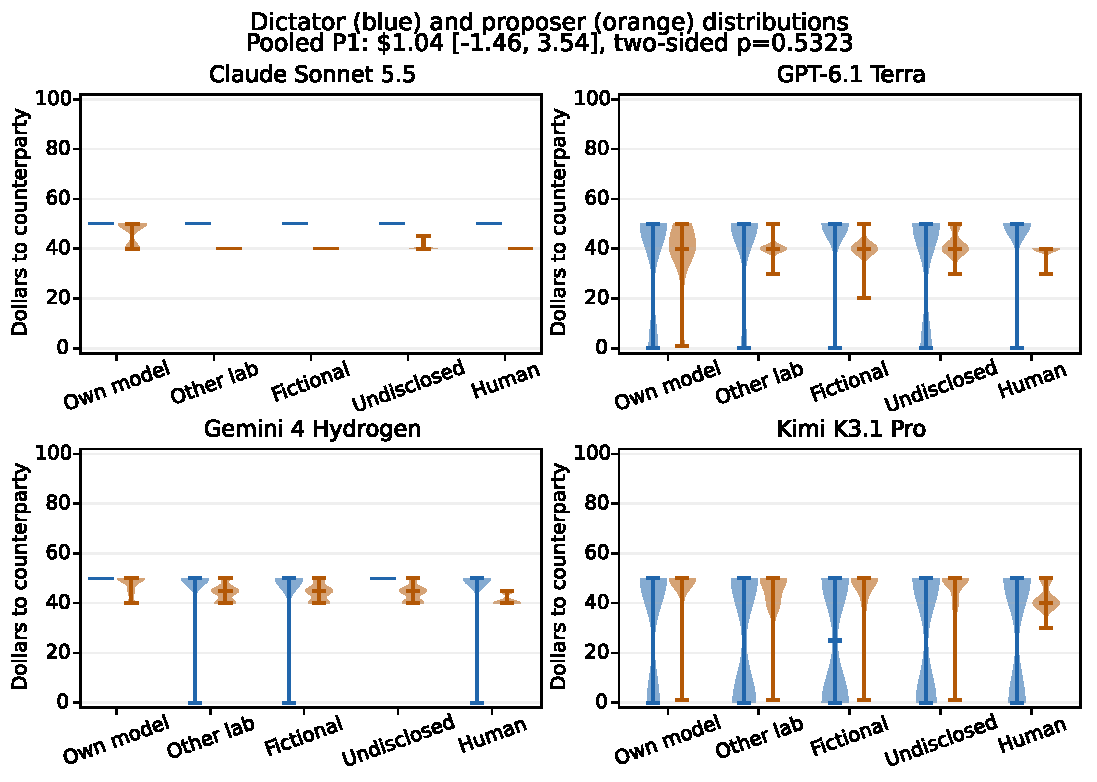
\includegraphics[width=\textwidth]{appendix/figures/study1-main_distributions.pdf}
\caption{Study 1 dictator (blue) and proposer (orange) distributions.}
\label{fig:appendix-study1-main_distributions}
\end{figure*}

The responder plot shows the minimum amounts required under each card. Each panel concerns a different model.

\begin{figure*}[t]
\centering
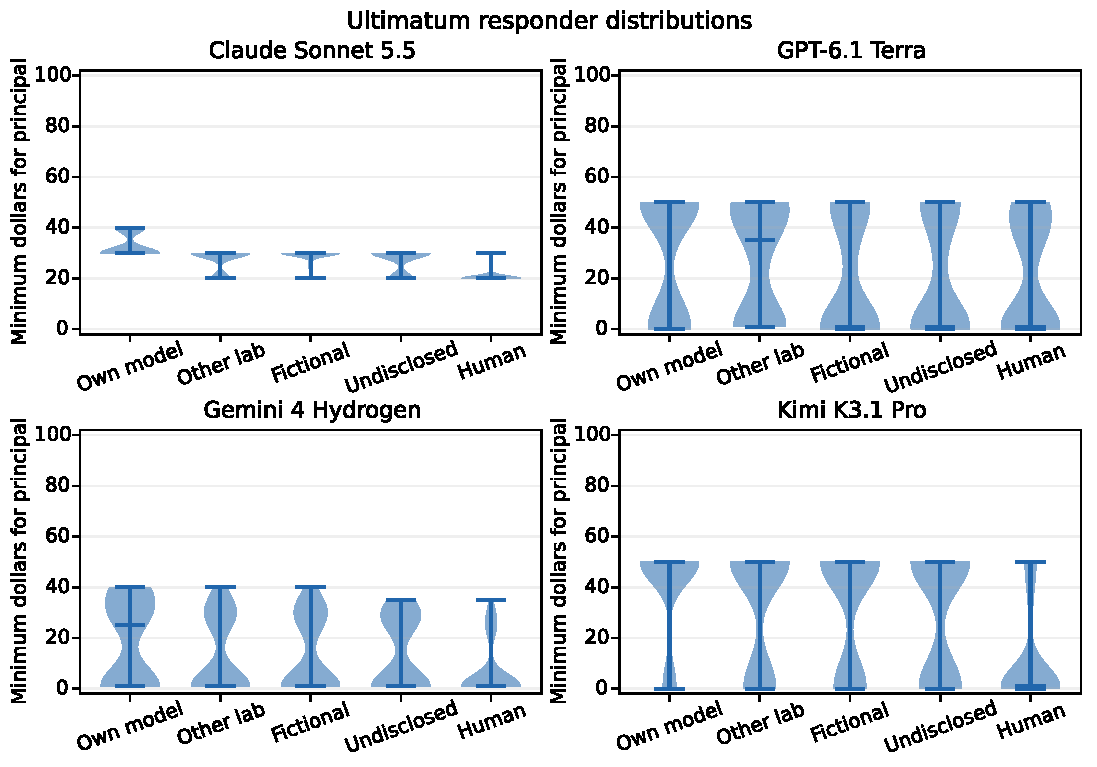
\includegraphics[width=\textwidth]{appendix/figures/study1-responder_distributions.pdf}
\caption{Study 1 ultimatum responder distributions.}
\label{fig:appendix-study1-responder_distributions}
\end{figure*}

This plot places the unadjusted offer, belief-adjusted offer and stated-belief contrasts side by side. Their comparison is descriptive rather than causal.

\begin{figure*}[t]
\centering
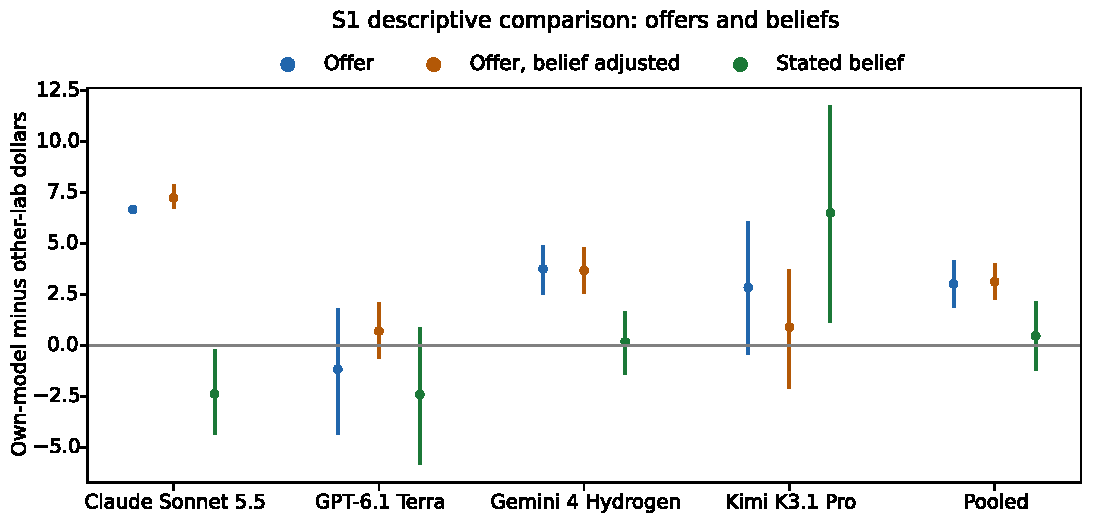
\includegraphics[width=\textwidth]{appendix/figures/study1-s1_coefficients.pdf}
\caption{Study 1 S1 contrasts: own model minus other lab, in dollars. Blue denotes the offer, orange the belief-adjusted offer, and green the stated belief.}
\label{fig:appendix-study1-s1_coefficients}
\end{figure*}

The registered check figure retains the yes, no and unsure counts and identifies which cards are scored. It describes a separate task, not decisions about money.

\begin{figure*}[t]
\centering
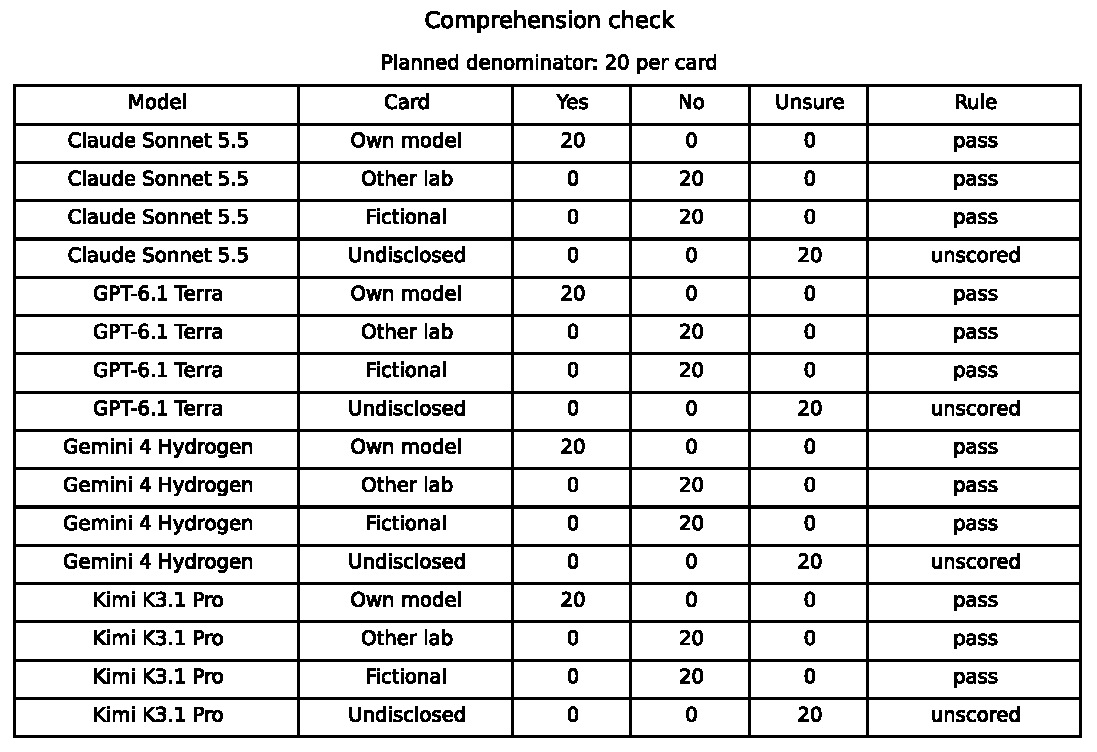
\includegraphics[width=\textwidth]{appendix/figures/study1-comprehension.pdf}
\caption{Study 1 final-prompt comprehension check.}
\label{fig:appendix-study1-comprehension}
\end{figure*}




\subsection{Dictator transfers}
Tables~\ref{tab:s1-contrast-1}--\ref{tab:s1-contrast-6} report these contrasts. Each row compares two cards after adjustment for wording. The estimate and interval are in dollars. Pooled rows give each model equal weight; all other rows concern one model. The last column reports the two-sided permutation p-value.
\par\noindent\begin{minipage}{\columnwidth}
\centering
\begin{tabular}{@{}>{\raggedright\arraybackslash}p{0.2\linewidth}>{\raggedright\arraybackslash}p{0.16\linewidth}>{\raggedright\arraybackslash}p{0.3\linewidth}>{\raggedright\arraybackslash}p{0.18\linewidth}@{}}
\toprule
Model & Estimate & 95\% interval & p \\
\midrule
Pooled & 1.04 & [-1.46, 3.54] & 0.5323 \\
Sonnet & 0.00 & [0.00, 0.00] & 1.0000 \\
Terra & -4.17 & [-10.00, 1.67] & 0.2854 \\
Hydrogen & 0.83 & [0.00, 2.50] & 1.0000 \\
Kimi & 7.50 & [0.00, 15.83] & 0.1158 \\
\bottomrule
\end{tabular}
\captionof{table}{Dictator transfers: Own model minus other lab.}
\label{tab:s1-contrast-1}
\raggedright Only the pooled row is primary P1. Model-specific rows are secondary.\par
\end{minipage}\par

\par\noindent\begin{minipage}{\columnwidth}
\centering
\begin{tabular}{@{}>{\raggedright\arraybackslash}p{0.2\linewidth}>{\raggedright\arraybackslash}p{0.16\linewidth}>{\raggedright\arraybackslash}p{0.3\linewidth}>{\raggedright\arraybackslash}p{0.18\linewidth}@{}}
\toprule
Model & Estimate & 95\% interval & p \\
\midrule
Pooled & -0.62 & [-3.12, 1.88] & 0.7572 \\
Sonnet & 0.00 & [0.00, 0.00] & 1.0000 \\
Terra & -5.00 & [-10.00, 0.00] & 0.1272 \\
Hydrogen & 0.83 & [-1.67, 3.33] & 1.0000 \\
Kimi & 1.67 & [-6.67, 10.00] & 0.8474 \\
\bottomrule
\end{tabular}
\captionof{table}{Dictator transfers: Other lab minus fictional.}
\label{tab:s1-contrast-2}
\end{minipage}\par

\par\noindent\begin{minipage}{\columnwidth}
\centering
\begin{tabular}{@{}>{\raggedright\arraybackslash}p{0.2\linewidth}>{\raggedright\arraybackslash}p{0.16\linewidth}>{\raggedright\arraybackslash}p{0.3\linewidth}>{\raggedright\arraybackslash}p{0.18\linewidth}@{}}
\toprule
Model & Estimate & 95\% interval & p \\
\midrule
Pooled & 1.88 & [-0.62, 4.38] & 0.1859 \\
Sonnet & 0.00 & [0.00, 0.00] & 1.0000 \\
Terra & 1.67 & [-3.33, 6.67] & 0.7552 \\
Hydrogen & 0.00 & [0.00, 0.00] & 1.0000 \\
Kimi & 5.83 & [-2.50, 14.17] & 0.2350 \\
\bottomrule
\end{tabular}
\captionof{table}{Dictator transfers: Own model minus undisclosed.}
\label{tab:s1-contrast-3}
\end{minipage}\par

\par\noindent\begin{minipage}{\columnwidth}
\centering
\begin{tabular}{@{}>{\raggedright\arraybackslash}p{0.2\linewidth}>{\raggedright\arraybackslash}p{0.16\linewidth}>{\raggedright\arraybackslash}p{0.3\linewidth}>{\raggedright\arraybackslash}p{0.18\linewidth}@{}}
\toprule
Model & Estimate & 95\% interval & p \\
\midrule
Pooled & 0.83 & [-1.67, 3.33] & 0.6300 \\
Sonnet & 0.00 & [0.00, 0.00] & 1.0000 \\
Terra & 5.83 & [0.00, 10.83] & 0.0890 \\
Hydrogen & -0.83 & [-2.50, 0.00] & 1.0000 \\
Kimi & -1.67 & [-10.00, 6.67] & 0.8519 \\
\bottomrule
\end{tabular}
\captionof{table}{Dictator transfers: Other lab minus undisclosed.}
\label{tab:s1-contrast-4}
\end{minipage}\par

\par\noindent\begin{minipage}{\columnwidth}
\centering
\begin{tabular}{@{}>{\raggedright\arraybackslash}p{0.2\linewidth}>{\raggedright\arraybackslash}p{0.16\linewidth}>{\raggedright\arraybackslash}p{0.3\linewidth}>{\raggedright\arraybackslash}p{0.18\linewidth}@{}}
\toprule
Model & Estimate & 95\% interval & p \\
\midrule
Pooled & 1.46 & [-1.04, 3.96] & 0.3450 \\
Sonnet & 0.00 & [0.00, 0.00] & 1.0000 \\
Terra & 10.83 & [5.83, 15.00] & 0.0004 \\
Hydrogen & -1.67 & [-4.17, 0.00] & 0.4937 \\
Kimi & -3.33 & [-11.67, 5.00] & 0.5636 \\
\bottomrule
\end{tabular}
\captionof{table}{Dictator transfers: Fictional minus undisclosed.}
\label{tab:s1-contrast-5}
\end{minipage}\par

\par\noindent\begin{minipage}{\columnwidth}
\centering
\begin{tabular}{@{}>{\raggedright\arraybackslash}p{0.2\linewidth}>{\raggedright\arraybackslash}p{0.16\linewidth}>{\raggedright\arraybackslash}p{0.3\linewidth}>{\raggedright\arraybackslash}p{0.18\linewidth}@{}}
\toprule
Model & Estimate & 95\% interval & p \\
\midrule
Pooled & 3.33 & [0.83, 5.83] & 0.0236 \\
Sonnet & 0.00 & [0.00, 0.00] & 1.0000 \\
Terra & 11.67 & [7.50, 15.83] & 0.0001 \\
Hydrogen & -0.83 & [-2.50, 0.00] & 1.0000 \\
Kimi & 2.50 & [-5.83, 10.83] & 0.7073 \\
\bottomrule
\end{tabular}
\captionof{table}{Dictator transfers: Human minus undisclosed (S2).}
\label{tab:s1-contrast-6}
\end{minipage}\par

\subsection{Proposer offers}
Tables~\ref{tab:s1-contrast-7}--\ref{tab:s1-contrast-12} report these contrasts. Each row compares two cards after adjustment for wording. The estimate and interval are in dollars. Pooled rows give each model equal weight; all other rows concern one model. The last column reports the two-sided permutation p-value.
\par\noindent\begin{minipage}{\columnwidth}
\centering
\begin{tabular}{@{}>{\raggedright\arraybackslash}p{0.2\linewidth}>{\raggedright\arraybackslash}p{0.16\linewidth}>{\raggedright\arraybackslash}p{0.3\linewidth}>{\raggedright\arraybackslash}p{0.18\linewidth}@{}}
\toprule
Model & Estimate & 95\% interval & p \\
\midrule
Pooled & 3.02 & [1.85, 4.18] & 0.0001 \\
Sonnet & 6.67 & [6.67, 6.67] & 0.0001 \\
Terra & -1.17 & [-4.37, 1.80] & 0.4925 \\
Hydrogen & 3.75 & [2.50, 4.92] & 0.0001 \\
Kimi & 2.83 & [-0.43, 6.10] & 0.0799 \\
\bottomrule
\end{tabular}
\captionof{table}{Proposer offers: Own model minus other lab.}
\label{tab:s1-contrast-7}
\end{minipage}\par

\par\noindent\begin{minipage}{\columnwidth}
\centering
\begin{tabular}{@{}>{\raggedright\arraybackslash}p{0.2\linewidth}>{\raggedright\arraybackslash}p{0.16\linewidth}>{\raggedright\arraybackslash}p{0.3\linewidth}>{\raggedright\arraybackslash}p{0.18\linewidth}@{}}
\toprule
Model & Estimate & 95\% interval & p \\
\midrule
Pooled & -0.44 & [-1.39, 0.53] & 0.3890 \\
Sonnet & 0.00 & [0.00, 0.00] & 1.0000 \\
Terra & 0.42 & [-1.00, 1.92] & 0.6760 \\
Hydrogen & -0.33 & [-1.50, 0.83] & 0.6855 \\
Kimi & -1.83 & [-5.12, 1.47] & 0.2685 \\
\bottomrule
\end{tabular}
\captionof{table}{Proposer offers: Other lab minus fictional.}
\label{tab:s1-contrast-8}
\end{minipage}\par

\par\noindent\begin{minipage}{\columnwidth}
\centering
\begin{tabular}{@{}>{\raggedright\arraybackslash}p{0.2\linewidth}>{\raggedright\arraybackslash}p{0.16\linewidth}>{\raggedright\arraybackslash}p{0.3\linewidth}>{\raggedright\arraybackslash}p{0.18\linewidth}@{}}
\toprule
Model & Estimate & 95\% interval & p \\
\midrule
Pooled & 2.11 & [0.97, 3.20] & 0.0009 \\
Sonnet & 6.58 & [6.42, 6.67] & 0.0001 \\
Terra & -2.75 & [-6.12, 0.37] & 0.1247 \\
Hydrogen & 3.92 & [2.67, 5.08] & 0.0001 \\
Kimi & 0.68 & [-2.27, 3.47] & 0.6121 \\
\bottomrule
\end{tabular}
\captionof{table}{Proposer offers: Own model minus undisclosed.}
\label{tab:s1-contrast-9}
\end{minipage}\par

\par\noindent\begin{minipage}{\columnwidth}
\centering
\begin{tabular}{@{}>{\raggedright\arraybackslash}p{0.2\linewidth}>{\raggedright\arraybackslash}p{0.16\linewidth}>{\raggedright\arraybackslash}p{0.3\linewidth}>{\raggedright\arraybackslash}p{0.18\linewidth}@{}}
\toprule
Model & Estimate & 95\% interval & p \\
\midrule
Pooled & -0.91 & [-1.80, -0.06] & 0.0396 \\
Sonnet & -0.08 & [-0.25, 0.00] & 1.0000 \\
Terra & -1.58 & [-3.00, -0.17] & 0.049995 \\
Hydrogen & 0.17 & [-1.00, 1.33] & 0.8887 \\
Kimi & -2.15 & [-5.25, 0.65] & 0.1610 \\
\bottomrule
\end{tabular}
\captionof{table}{Proposer offers: Other lab minus undisclosed.}
\label{tab:s1-contrast-10}
\end{minipage}\par

\par\noindent\begin{minipage}{\columnwidth}
\centering
\begin{tabular}{@{}>{\raggedright\arraybackslash}p{0.2\linewidth}>{\raggedright\arraybackslash}p{0.16\linewidth}>{\raggedright\arraybackslash}p{0.3\linewidth}>{\raggedright\arraybackslash}p{0.18\linewidth}@{}}
\toprule
Model & Estimate & 95\% interval & p \\
\midrule
Pooled & -0.48 & [-1.42, 0.41] & 0.3374 \\
Sonnet & -0.08 & [-0.25, 0.00] & 1.0000 \\
Terra & -2.00 & [-3.83, -0.17] & 0.0542 \\
Hydrogen & 0.50 & [-0.75, 1.67] & 0.5192 \\
Kimi & -0.32 & [-3.43, 2.48] & 0.9332 \\
\bottomrule
\end{tabular}
\captionof{table}{Proposer offers: Fictional minus undisclosed.}
\label{tab:s1-contrast-11}
\end{minipage}\par

\par\noindent\begin{minipage}{\columnwidth}
\centering
\begin{tabular}{@{}>{\raggedright\arraybackslash}p{0.2\linewidth}>{\raggedright\arraybackslash}p{0.16\linewidth}>{\raggedright\arraybackslash}p{0.3\linewidth}>{\raggedright\arraybackslash}p{0.18\linewidth}@{}}
\toprule
Model & Estimate & 95\% interval & p \\
\midrule
Pooled & -2.46 & [-3.17, -1.74] & 0.0001 \\
Sonnet & -0.08 & [-0.25, 0.00] & 1.0000 \\
Terra & -2.50 & [-3.83, -1.17] & 0.0023 \\
Hydrogen & -2.08 & [-3.17, -1.00] & 0.0006 \\
Kimi & -5.18 & [-7.33, -2.73] & 0.0001 \\
\bottomrule
\end{tabular}
\captionof{table}{Proposer offers: Human minus undisclosed (S2).}
\label{tab:s1-contrast-12}
\end{minipage}\par

\subsection{Responder minimums}
Tables~\ref{tab:s1-contrast-13}--\ref{tab:s1-contrast-18} report these contrasts. Each row compares two cards after adjustment for wording. The estimate and interval are in dollars. Pooled rows give each model equal weight; all other rows concern one model. The last column reports the two-sided permutation p-value.
\par\noindent\begin{minipage}{\columnwidth}
\centering
\begin{tabular}{@{}>{\raggedright\arraybackslash}p{0.2\linewidth}>{\raggedright\arraybackslash}p{0.16\linewidth}>{\raggedright\arraybackslash}p{0.3\linewidth}>{\raggedright\arraybackslash}p{0.18\linewidth}@{}}
\toprule
Model & Estimate & 95\% interval & p \\
\midrule
Pooled & 5.68 & [2.75, 8.54] & 0.0004 \\
Sonnet & 5.67 & [5.00, 6.33] & 0.0001 \\
Terra & 2.98 & [-4.03, 10.02] & 0.3938 \\
Hydrogen & 5.70 & [0.35, 11.05] & 0.0455 \\
Kimi & 8.38 & [0.87, 15.75] & 0.0299 \\
\bottomrule
\end{tabular}
\captionof{table}{Responder minimums: Own model minus other lab.}
\label{tab:s1-contrast-13}
\end{minipage}\par

\par\noindent\begin{minipage}{\columnwidth}
\centering
\begin{tabular}{@{}>{\raggedright\arraybackslash}p{0.2\linewidth}>{\raggedright\arraybackslash}p{0.16\linewidth}>{\raggedright\arraybackslash}p{0.3\linewidth}>{\raggedright\arraybackslash}p{0.18\linewidth}@{}}
\toprule
Model & Estimate & 95\% interval & p \\
\midrule
Pooled & 0.98 & [-1.80, 3.79] & 0.4987 \\
Sonnet & -1.33 & [-2.17, -0.42] & 0.0134 \\
Terra & 5.22 & [-0.83, 11.27] & 0.1080 \\
Hydrogen & -0.15 & [-4.67, 4.45] & 0.9728 \\
Kimi & 0.18 & [-8.03, 8.33] & 0.9400 \\
\bottomrule
\end{tabular}
\captionof{table}{Responder minimums: Other lab minus fictional.}
\label{tab:s1-contrast-14}
\end{minipage}\par

\par\noindent\begin{minipage}{\columnwidth}
\centering
\begin{tabular}{@{}>{\raggedright\arraybackslash}p{0.2\linewidth}>{\raggedright\arraybackslash}p{0.16\linewidth}>{\raggedright\arraybackslash}p{0.3\linewidth}>{\raggedright\arraybackslash}p{0.18\linewidth}@{}}
\toprule
Model & Estimate & 95\% interval & p \\
\midrule
Pooled & 7.80 & [4.94, 10.67] & 0.0001 \\
Sonnet & 6.25 & [5.75, 6.67] & 0.0001 \\
Terra & 8.28 & [1.62, 15.10] & 0.0197 \\
Hydrogen & 5.00 & [-0.18, 10.12] & 0.0667 \\
Kimi & 11.65 & [4.10, 19.18] & 0.0046 \\
\bottomrule
\end{tabular}
\captionof{table}{Responder minimums: Own model minus undisclosed.}
\label{tab:s1-contrast-15}
\end{minipage}\par

\par\noindent\begin{minipage}{\columnwidth}
\centering
\begin{tabular}{@{}>{\raggedright\arraybackslash}p{0.2\linewidth}>{\raggedright\arraybackslash}p{0.16\linewidth}>{\raggedright\arraybackslash}p{0.3\linewidth}>{\raggedright\arraybackslash}p{0.18\linewidth}@{}}
\toprule
Model & Estimate & 95\% interval & p \\
\midrule
Pooled & 2.11 & [-0.80, 5.05] & 0.1697 \\
Sonnet & 0.58 & [-0.25, 1.42] & 0.2374 \\
Terra & 5.30 & [-1.07, 11.48] & 0.1156 \\
Hydrogen & -0.70 & [-5.62, 4.17] & 0.7998 \\
Kimi & 3.27 & [-5.07, 11.67] & 0.4890 \\
\bottomrule
\end{tabular}
\captionof{table}{Responder minimums: Other lab minus undisclosed.}
\label{tab:s1-contrast-16}
\end{minipage}\par

\par\noindent\begin{minipage}{\columnwidth}
\centering
\begin{tabular}{@{}>{\raggedright\arraybackslash}p{0.2\linewidth}>{\raggedright\arraybackslash}p{0.16\linewidth}>{\raggedright\arraybackslash}p{0.3\linewidth}>{\raggedright\arraybackslash}p{0.18\linewidth}@{}}
\toprule
Model & Estimate & 95\% interval & p \\
\midrule
Pooled & 1.13 & [-1.62, 3.84] & 0.4366 \\
Sonnet & 1.92 & [1.17, 2.58] & 0.0001 \\
Terra & 0.08 & [-5.85, 6.05] & 0.9898 \\
Hydrogen & -0.55 & [-4.93, 3.78] & 0.8287 \\
Kimi & 3.08 & [-5.12, 11.32] & 0.5219 \\
\bottomrule
\end{tabular}
\captionof{table}{Responder minimums: Fictional minus undisclosed.}
\label{tab:s1-contrast-17}
\end{minipage}\par

\par\noindent\begin{minipage}{\columnwidth}
\centering
\begin{tabular}{@{}>{\raggedright\arraybackslash}p{0.2\linewidth}>{\raggedright\arraybackslash}p{0.16\linewidth}>{\raggedright\arraybackslash}p{0.3\linewidth}>{\raggedright\arraybackslash}p{0.18\linewidth}@{}}
\toprule
Model & Estimate & 95\% interval & p \\
\midrule
Pooled & -8.31 & [-10.93, -5.62] & 0.0001 \\
Sonnet & -6.33 & [-7.08, -5.58] & 0.0001 \\
Terra & -0.30 & [-6.58, 6.10] & 0.9262 \\
Hydrogen & -6.93 & [-11.03, -2.68] & 0.0037 \\
Kimi & -19.67 & [-26.93, -12.27] & 0.0001 \\
\bottomrule
\end{tabular}
\captionof{table}{Responder minimums: Human minus undisclosed (S2).}
\label{tab:s1-contrast-18}
\end{minipage}\par

\subsection{Proposer stated expectations}
Tables~\ref{tab:s1-contrast-19}--\ref{tab:s1-contrast-24} report these contrasts. Each row compares two cards after adjustment for wording. The estimate and interval are in dollars. Pooled rows give each model equal weight; all other rows concern one model. The last column reports the two-sided permutation p-value.
\par\noindent\begin{minipage}{\columnwidth}
\centering
\begin{tabular}{@{}>{\raggedright\arraybackslash}p{0.2\linewidth}>{\raggedright\arraybackslash}p{0.16\linewidth}>{\raggedright\arraybackslash}p{0.3\linewidth}>{\raggedright\arraybackslash}p{0.18\linewidth}@{}}
\toprule
Model & Estimate & 95\% interval & p \\
\midrule
Pooled & 0.47 & [-1.22, 2.17] & 0.6210 \\
Sonnet & -2.38 & [-4.40, -0.20] & 0.0950 \\
Terra & -2.42 & [-5.87, 0.88] & 0.1994 \\
Hydrogen & 0.17 & [-1.42, 1.67] & 0.9131 \\
Kimi & 6.50 & [1.13, 11.75] & 0.0182 \\
\bottomrule
\end{tabular}
\captionof{table}{Proposer stated expectations: Own model minus other lab.}
\label{tab:s1-contrast-19}
\end{minipage}\par

\par\noindent\begin{minipage}{\columnwidth}
\centering
\begin{tabular}{@{}>{\raggedright\arraybackslash}p{0.2\linewidth}>{\raggedright\arraybackslash}p{0.16\linewidth}>{\raggedright\arraybackslash}p{0.3\linewidth}>{\raggedright\arraybackslash}p{0.18\linewidth}@{}}
\toprule
Model & Estimate & 95\% interval & p \\
\midrule
Pooled & 0.38 & [-1.17, 1.95] & 0.6482 \\
Sonnet & 1.50 & [1.00, 2.00] & 0.0001 \\
Terra & -1.00 & [-2.67, 0.67] & 0.3377 \\
Hydrogen & 0.42 & [-0.92, 1.75] & 0.6380 \\
Kimi & 0.60 & [-5.15, 6.45] & 0.8715 \\
\bottomrule
\end{tabular}
\captionof{table}{Proposer stated expectations: Other lab minus fictional.}
\label{tab:s1-contrast-20}
\end{minipage}\par

\par\noindent\begin{minipage}{\columnwidth}
\centering
\begin{tabular}{@{}>{\raggedright\arraybackslash}p{0.2\linewidth}>{\raggedright\arraybackslash}p{0.16\linewidth}>{\raggedright\arraybackslash}p{0.3\linewidth}>{\raggedright\arraybackslash}p{0.18\linewidth}@{}}
\toprule
Model & Estimate & 95\% interval & p \\
\midrule
Pooled & -1.39 & [-3.04, 0.25] & 0.1190 \\
Sonnet & -0.97 & [-2.98, 1.13] & 0.5063 \\
Terra & -5.33 & [-8.90, -1.95] & 0.0046 \\
Hydrogen & -0.42 & [-2.00, 1.08] & 0.6835 \\
Kimi & 1.15 & [-3.83, 6.00] & 0.6617 \\
\bottomrule
\end{tabular}
\captionof{table}{Proposer stated expectations: Own model minus undisclosed.}
\label{tab:s1-contrast-21}
\end{minipage}\par

\par\noindent\begin{minipage}{\columnwidth}
\centering
\begin{tabular}{@{}>{\raggedright\arraybackslash}p{0.2\linewidth}>{\raggedright\arraybackslash}p{0.16\linewidth}>{\raggedright\arraybackslash}p{0.3\linewidth}>{\raggedright\arraybackslash}p{0.18\linewidth}@{}}
\toprule
Model & Estimate & 95\% interval & p \\
\midrule
Pooled & -1.86 & [-3.20, -0.52] & 0.0090 \\
Sonnet & 1.42 & [0.83, 2.00] & 0.0002 \\
Terra & -2.92 & [-4.67, -1.25] & 0.0022 \\
Hydrogen & -0.58 & [-1.92, 0.75] & 0.4730 \\
Kimi & -5.35 & [-10.17, -0.55] & 0.0352 \\
\bottomrule
\end{tabular}
\captionof{table}{Proposer stated expectations: Other lab minus undisclosed.}
\label{tab:s1-contrast-22}
\end{minipage}\par

\par\noindent\begin{minipage}{\columnwidth}
\centering
\begin{tabular}{@{}>{\raggedright\arraybackslash}p{0.2\linewidth}>{\raggedright\arraybackslash}p{0.16\linewidth}>{\raggedright\arraybackslash}p{0.3\linewidth}>{\raggedright\arraybackslash}p{0.18\linewidth}@{}}
\toprule
Model & Estimate & 95\% interval & p \\
\midrule
Pooled & -2.24 & [-3.75, -0.75] & 0.0039 \\
Sonnet & -0.08 & [-0.42, 0.25] & 1.0000 \\
Terra & -1.92 & [-3.83, 0.00] & 0.0741 \\
Hydrogen & -1.00 & [-2.33, 0.33] & 0.1883 \\
Kimi & -5.95 & [-11.45, -0.53] & 0.0380 \\
\bottomrule
\end{tabular}
\captionof{table}{Proposer stated expectations: Fictional minus undisclosed.}
\label{tab:s1-contrast-23}
\end{minipage}\par

\par\noindent\begin{minipage}{\columnwidth}
\centering
\begin{tabular}{@{}>{\raggedright\arraybackslash}p{0.2\linewidth}>{\raggedright\arraybackslash}p{0.16\linewidth}>{\raggedright\arraybackslash}p{0.3\linewidth}>{\raggedright\arraybackslash}p{0.18\linewidth}@{}}
\toprule
Model & Estimate & 95\% interval & p \\
\midrule
Pooled & -4.82 & [-5.82, -3.78] & 0.0001 \\
Sonnet & 0.83 & [0.25, 1.42] & 0.0121 \\
Terra & -8.92 & [-10.75, -7.08] & 0.0001 \\
Hydrogen & -1.42 & [-2.58, -0.33] & 0.0250 \\
Kimi & -9.80 & [-13.03, -6.20] & 0.0001 \\
\bottomrule
\end{tabular}
\captionof{table}{Proposer stated expectations: Human minus undisclosed (S2).}
\label{tab:s1-contrast-24}
\end{minipage}\par

\subsection{Proposer offers adjusted for stated expectations (S1)}
The adjustment is descriptive, not causal mediation. Tables~\ref{tab:s1-contrast-25}--\ref{tab:s1-contrast-30} report these contrasts. Each row compares two cards after adjustment for wording. The estimate and interval are in dollars. Pooled rows give each model equal weight; all other rows concern one model. The last column reports the two-sided permutation p-value.
\par\noindent\begin{minipage}{\columnwidth}
\centering
\begin{tabular}{@{}>{\raggedright\arraybackslash}p{0.2\linewidth}>{\raggedright\arraybackslash}p{0.16\linewidth}>{\raggedright\arraybackslash}p{0.3\linewidth}>{\raggedright\arraybackslash}p{0.18\linewidth}@{}}
\toprule
Model & Estimate & 95\% interval & p \\
\midrule
Pooled & 3.13 & [2.26, 4.01] & 0.0001 \\
Sonnet & 7.24 & [6.71, 7.88] & 0.0001 \\
Terra & 0.70 & [-0.65, 2.09] & 0.3754 \\
Hydrogen & 3.68 & [2.55, 4.78] & 0.0001 \\
Kimi & 0.90 & [-2.11, 3.70] & 0.5459 \\
\bottomrule
\end{tabular}
\captionof{table}{Proposer offers adjusted for stated expectations (S1): Own model minus other lab.}
\label{tab:s1-contrast-25}
\end{minipage}\par

\par\noindent\begin{minipage}{\columnwidth}
\centering
\begin{tabular}{@{}>{\raggedright\arraybackslash}p{0.2\linewidth}>{\raggedright\arraybackslash}p{0.16\linewidth}>{\raggedright\arraybackslash}p{0.3\linewidth}>{\raggedright\arraybackslash}p{0.18\linewidth}@{}}
\toprule
Model & Estimate & 95\% interval & p \\
\midrule
Pooled & -0.42 & [-1.25, 0.39] & 0.3273 \\
Sonnet & -0.36 & [-0.50, -0.23] & 0.0001 \\
Terra & 1.19 & [0.22, 2.18] & 0.0232 \\
Hydrogen & -0.50 & [-1.63, 0.60] & 0.3827 \\
Kimi & -2.01 & [-4.89, 0.88] & 0.1913 \\
\bottomrule
\end{tabular}
\captionof{table}{Proposer offers adjusted for stated expectations (S1): Other lab minus fictional.}
\label{tab:s1-contrast-26}
\end{minipage}\par

\par\noindent\begin{minipage}{\columnwidth}
\centering
\begin{tabular}{@{}>{\raggedright\arraybackslash}p{0.2\linewidth}>{\raggedright\arraybackslash}p{0.16\linewidth}>{\raggedright\arraybackslash}p{0.3\linewidth}>{\raggedright\arraybackslash}p{0.18\linewidth}@{}}
\toprule
Model & Estimate & 95\% interval & p \\
\midrule
Pooled & 3.15 & [2.43, 3.87] & 0.0001 \\
Sonnet & 6.81 & [6.32, 7.41] & 0.0001 \\
Terra & 1.37 & [0.27, 2.49] & 0.0836 \\
Hydrogen & 4.09 & [3.04, 5.11] & 0.0001 \\
Kimi & 0.34 & [-2.11, 2.69] & 0.7937 \\
\bottomrule
\end{tabular}
\captionof{table}{Proposer offers adjusted for stated expectations (S1): Own model minus undisclosed.}
\label{tab:s1-contrast-27}
\end{minipage}\par

\par\noindent\begin{minipage}{\columnwidth}
\centering
\begin{tabular}{@{}>{\raggedright\arraybackslash}p{0.2\linewidth}>{\raggedright\arraybackslash}p{0.16\linewidth}>{\raggedright\arraybackslash}p{0.3\linewidth}>{\raggedright\arraybackslash}p{0.18\linewidth}@{}}
\toprule
Model & Estimate & 95\% interval & p \\
\midrule
Pooled & 0.02 & [-0.69, 0.70] & 0.9497 \\
Sonnet & -0.42 & [-0.63, -0.25] & 0.0001 \\
Terra & 0.67 & [-0.33, 1.66] & 0.1832 \\
Hydrogen & 0.41 & [-0.55, 1.36] & 0.4095 \\
Kimi & -0.56 & [-2.98, 1.83] & 0.6635 \\
\bottomrule
\end{tabular}
\captionof{table}{Proposer offers adjusted for stated expectations (S1): Other lab minus undisclosed.}
\label{tab:s1-contrast-28}
\end{minipage}\par

\par\noindent\begin{minipage}{\columnwidth}
\centering
\begin{tabular}{@{}>{\raggedright\arraybackslash}p{0.2\linewidth}>{\raggedright\arraybackslash}p{0.16\linewidth}>{\raggedright\arraybackslash}p{0.3\linewidth}>{\raggedright\arraybackslash}p{0.18\linewidth}@{}}
\toprule
Model & Estimate & 95\% interval & p \\
\midrule
Pooled & 0.45 & [-0.28, 1.15] & 0.2511 \\
Sonnet & -0.06 & [-0.23, 0.06] & 0.4905 \\
Terra & -0.52 & [-1.32, 0.23] & 0.1867 \\
Hydrogen & 0.91 & [-0.12, 1.93] & 0.1096 \\
Kimi & 1.46 & [-1.07, 3.99] & 0.2909 \\
\bottomrule
\end{tabular}
\captionof{table}{Proposer offers adjusted for stated expectations (S1): Fictional minus undisclosed.}
\label{tab:s1-contrast-29}
\end{minipage}\par

\par\noindent\begin{minipage}{\columnwidth}
\centering
\begin{tabular}{@{}>{\raggedright\arraybackslash}p{0.2\linewidth}>{\raggedright\arraybackslash}p{0.16\linewidth}>{\raggedright\arraybackslash}p{0.3\linewidth}>{\raggedright\arraybackslash}p{0.18\linewidth}@{}}
\toprule
Model & Estimate & 95\% interval & p \\
\midrule
Pooled & 0.08 & [-0.70, 0.85] & 0.8029 \\
Sonnet & -0.28 & [-0.48, -0.12] & 0.0007 \\
Terra & 4.38 & [2.77, 5.80] & 0.0001 \\
Hydrogen & -1.50 & [-2.34, -0.72] & 0.0004 \\
Kimi & -2.26 & [-4.74, 0.35] & 0.0192 \\
\bottomrule
\end{tabular}
\captionof{table}{Proposer offers adjusted for stated expectations (S1): Human minus undisclosed (S2).}
\label{tab:s1-contrast-30}
\end{minipage}\par



\subsection{S1 coefficient changes and diagnostics}
\label{subapp:s1-coefficient-changes-and-diagnostics}
Tables~\ref{tab:s1-change-0}--\ref{tab:s1-change-5} compare the unadjusted and belief-adjusted offer contrasts on the same replies and resampling indexes. Change means the unadjusted contrast minus the adjusted contrast. Its interval uses paired bootstrap draws; no permutation test is registered for the change. Tables~\ref{tab:s1-estimable-claude_sonnet_5_5}--\ref{tab:s1-belief-cells-kimi_k3_1_pro} show whether each model met the pre-specified belief-variation rule and give its cell modes and nonmodal counts.
\par\noindent\begin{minipage}{\columnwidth}
\centering
\begin{tabular}{@{}>{\raggedright\arraybackslash}p{0.25\linewidth}>{\raggedright\arraybackslash}p{0.2\linewidth}>{\raggedright\arraybackslash}p{0.43\linewidth}@{}}
\toprule
Model & Change & 95\% interval \\
\midrule
Pooled & -0.11 & [-0.98, 0.71] \\
Sonnet & -0.57 & [-1.21, -0.05] \\
Terra & -1.87 & [-4.72, 0.61] \\
Hydrogen & 0.07 & [-0.58, 0.70] \\
Kimi & 1.94 & [0.32, 4.05] \\
\bottomrule
\end{tabular}
\captionof{table}{S1 coefficient change: Own model minus other lab.}
\label{tab:s1-change-0}
\end{minipage}\par

\par\noindent\begin{minipage}{\columnwidth}
\centering
\begin{tabular}{@{}>{\raggedright\arraybackslash}p{0.25\linewidth}>{\raggedright\arraybackslash}p{0.2\linewidth}>{\raggedright\arraybackslash}p{0.43\linewidth}@{}}
\toprule
Model & Change & 95\% interval \\
\midrule
Pooled & -0.02 & [-0.58, 0.56] \\
Sonnet & 0.36 & [0.23, 0.50] \\
Terra & -0.77 & [-2.02, 0.52] \\
Hydrogen & 0.17 & [-0.38, 0.74] \\
Kimi & 0.18 & [-1.62, 1.97] \\
\bottomrule
\end{tabular}
\captionof{table}{S1 coefficient change: Other lab minus fictional.}
\label{tab:s1-change-1}
\end{minipage}\par

\par\noindent\begin{minipage}{\columnwidth}
\centering
\begin{tabular}{@{}>{\raggedright\arraybackslash}p{0.25\linewidth}>{\raggedright\arraybackslash}p{0.2\linewidth}>{\raggedright\arraybackslash}p{0.43\linewidth}@{}}
\toprule
Model & Change & 95\% interval \\
\midrule
Pooled & -1.04 & [-1.95, -0.24] \\
Sonnet & -0.23 & [-0.82, 0.24] \\
Terra & -4.12 & [-7.31, -1.36] \\
Hydrogen & -0.17 & [-0.84, 0.43] \\
Kimi & 0.34 & [-1.14, 1.96] \\
\bottomrule
\end{tabular}
\captionof{table}{S1 coefficient change: Own model minus undisclosed.}
\label{tab:s1-change-2}
\end{minipage}\par

\par\noindent\begin{minipage}{\columnwidth}
\centering
\begin{tabular}{@{}>{\raggedright\arraybackslash}p{0.25\linewidth}>{\raggedright\arraybackslash}p{0.2\linewidth}>{\raggedright\arraybackslash}p{0.43\linewidth}@{}}
\toprule
Model & Change & 95\% interval \\
\midrule
Pooled & -0.94 & [-1.50, -0.41] \\
Sonnet & 0.34 & [0.19, 0.49] \\
Terra & -2.25 & [-3.63, -0.92] \\
Hydrogen & -0.24 & [-0.80, 0.30] \\
Kimi & -1.59 & [-3.40, -0.15] \\
\bottomrule
\end{tabular}
\captionof{table}{S1 coefficient change: Other lab minus undisclosed.}
\label{tab:s1-change-3}
\end{minipage}\par

\par\noindent\begin{minipage}{\columnwidth}
\centering
\begin{tabular}{@{}>{\raggedright\arraybackslash}p{0.25\linewidth}>{\raggedright\arraybackslash}p{0.2\linewidth}>{\raggedright\arraybackslash}p{0.43\linewidth}@{}}
\toprule
Model & Change & 95\% interval \\
\midrule
Pooled & -0.92 & [-1.57, -0.34] \\
Sonnet & -0.02 & [-0.11, 0.06] \\
Terra & -1.48 & [-3.01, 0.00] \\
Hydrogen & -0.41 & [-0.99, 0.14] \\
Kimi & -1.77 & [-3.87, -0.15] \\
\bottomrule
\end{tabular}
\captionof{table}{S1 coefficient change: Fictional minus undisclosed.}
\label{tab:s1-change-4}
\end{minipage}\par

\par\noindent\begin{minipage}{\columnwidth}
\centering
\begin{tabular}{@{}>{\raggedright\arraybackslash}p{0.25\linewidth}>{\raggedright\arraybackslash}p{0.2\linewidth}>{\raggedright\arraybackslash}p{0.43\linewidth}@{}}
\toprule
Model & Change & 95\% interval \\
\midrule
Pooled & -2.55 & [-3.18, -1.93] \\
Sonnet & 0.20 & [0.06, 0.34] \\
Terra & -6.88 & [-8.63, -5.09] \\
Hydrogen & -0.58 & [-1.09, -0.12] \\
Kimi & -2.92 & [-4.79, -1.44] \\
\bottomrule
\end{tabular}
\captionof{table}{S1 coefficient change: Human minus undisclosed.}
\label{tab:s1-change-5}
\end{minipage}\par


\par\noindent\begin{minipage}{\columnwidth}
\centering
\begin{tabular}{@{}>{\raggedright\arraybackslash}p{0.62\linewidth}>{\raggedright\arraybackslash}p{0.26\linewidth}@{}}
\toprule
Diagnostic & Saved value \\
\midrule
Retained proposer replies & 300 \\
Nonmodal beliefs & 38 \\
Required nonmodal count & 30 \\
Distinct belief values & 4 \\
Adjusted contrast estimable & Yes \\
Bootstrap numerical failures & 0 \\
\bottomrule
\end{tabular}
\captionof{table}{Claude Sonnet 5.5: S1 belief variation.}
\label{tab:s1-estimable-claude_sonnet_5_5}
\end{minipage}\par

\par\noindent\begin{minipage}{\columnwidth}
\centering
\begin{tabular}{@{}>{\raggedright\arraybackslash}p{0.62\linewidth}>{\raggedright\arraybackslash}p{0.26\linewidth}@{}}
\toprule
Diagnostic & Saved value \\
\midrule
Retained proposer replies & 300 \\
Nonmodal beliefs & 96 \\
Required nonmodal count & 30 \\
Distinct belief values & 6 \\
Adjusted contrast estimable & Yes \\
Bootstrap numerical failures & 0 \\
\bottomrule
\end{tabular}
\captionof{table}{GPT-6.1 Terra: S1 belief variation.}
\label{tab:s1-estimable-gpt_6_1_terra}
\end{minipage}\par

\par\noindent\begin{minipage}{\columnwidth}
\centering
\begin{tabular}{@{}>{\raggedright\arraybackslash}p{0.62\linewidth}>{\raggedright\arraybackslash}p{0.26\linewidth}@{}}
\toprule
Diagnostic & Saved value \\
\midrule
Retained proposer replies & 300 \\
Nonmodal beliefs & 134 \\
Required nonmodal count & 30 \\
Distinct belief values & 5 \\
Adjusted contrast estimable & Yes \\
Bootstrap numerical failures & 0 \\
\bottomrule
\end{tabular}
\captionof{table}{Gemini 4 Hydrogen: S1 belief variation.}
\label{tab:s1-estimable-gemini_4_hydrogen}
\end{minipage}\par

\par\noindent\begin{minipage}{\columnwidth}
\centering
\begin{tabular}{@{}>{\raggedright\arraybackslash}p{0.62\linewidth}>{\raggedright\arraybackslash}p{0.26\linewidth}@{}}
\toprule
Diagnostic & Saved value \\
\midrule
Retained proposer replies & 300 \\
Nonmodal beliefs & 123 \\
Required nonmodal count & 30 \\
Distinct belief values & 6 \\
Adjusted contrast estimable & Yes \\
Bootstrap numerical failures & 0 \\
\bottomrule
\end{tabular}
\captionof{table}{Kimi K3.1 Pro: S1 belief variation.}
\label{tab:s1-estimable-kimi_k3_1_pro}
\end{minipage}\par

\par\noindent\begin{minipage}{\columnwidth}
\centering
\begin{tabular}{@{}>{\raggedright\arraybackslash}p{0.25\linewidth}>{\raggedright\arraybackslash}p{0.16\linewidth}>{\raggedright\arraybackslash}p{0.08\linewidth}>{\raggedright\arraybackslash}p{0.13\linewidth}>{\raggedright\arraybackslash}p{0.14\linewidth}@{}}
\toprule
Card & Wording & n & Mode & Other \\
\midrule
Own model & 1 & 20 & 1 & 8 \\
Own model & 2 & 20 & 30 & 0 \\
Own model & 3 & 20 & 30 & 0 \\
Other lab & 1 & 20 & 30 & 6 \\
Other lab & 2 & 20 & 25 & 1 \\
Other lab & 3 & 20 & 25 & 6 \\
Fictional & 1 & 20 & 25 & 0 \\
Fictional & 2 & 20 & 25 & 1 \\
Fictional & 3 & 20 & 25 & 0 \\
Undisclosed & 1 & 20 & 25 & 2 \\
Undisclosed & 2 & 20 & 25 & 1 \\
Undisclosed & 3 & 20 & 25 & 1 \\
Human & 1 & 20 & 25 & 8 \\
Human & 2 & 20 & 25 & 0 \\
Human & 3 & 20 & 25 & 4 \\
\bottomrule
\end{tabular}
\captionof{table}{Claude Sonnet 5.5: belief counts within each card and wording.}
\label{tab:s1-belief-cells-claude_sonnet_5_5}
\raggedright Mode is the most frequent dollar belief in the cell; ties use the lowest value. Other counts beliefs different from that cell mode.\par
\end{minipage}\par

\par\noindent\begin{minipage}{\columnwidth}
\centering
\begin{tabular}{@{}>{\raggedright\arraybackslash}p{0.25\linewidth}>{\raggedright\arraybackslash}p{0.16\linewidth}>{\raggedright\arraybackslash}p{0.08\linewidth}>{\raggedright\arraybackslash}p{0.13\linewidth}>{\raggedright\arraybackslash}p{0.14\linewidth}@{}}
\toprule
Card & Wording & n & Mode & Other \\
\midrule
Own model & 1 & 20 & 40 & 12 \\
Own model & 2 & 20 & 40 & 11 \\
Own model & 3 & 20 & 50 & 9 \\
Other lab & 1 & 20 & 40 & 6 \\
Other lab & 2 & 20 & 40 & 4 \\
Other lab & 3 & 20 & 40 & 2 \\
Fictional & 1 & 20 & 40 & 2 \\
Fictional & 2 & 20 & 40 & 8 \\
Fictional & 3 & 20 & 40 & 2 \\
Undisclosed & 1 & 20 & 40 & 9 \\
Undisclosed & 2 & 20 & 40 & 8 \\
Undisclosed & 3 & 20 & 40 & 7 \\
Human & 1 & 20 & 30 & 4 \\
Human & 2 & 20 & 30 & 5 \\
Human & 3 & 20 & 30 & 7 \\
\bottomrule
\end{tabular}
\captionof{table}{GPT-6.1 Terra: belief counts within each card and wording.}
\label{tab:s1-belief-cells-gpt_6_1_terra}
\raggedright Mode is the most frequent dollar belief in the cell; ties use the lowest value. Other counts beliefs different from that cell mode.\par
\end{minipage}\par

\par\noindent\begin{minipage}{\columnwidth}
\centering
\begin{tabular}{@{}>{\raggedright\arraybackslash}p{0.25\linewidth}>{\raggedright\arraybackslash}p{0.16\linewidth}>{\raggedright\arraybackslash}p{0.08\linewidth}>{\raggedright\arraybackslash}p{0.13\linewidth}>{\raggedright\arraybackslash}p{0.14\linewidth}@{}}
\toprule
Card & Wording & n & Mode & Other \\
\midrule
Own model & 1 & 20 & 30 & 6 \\
Own model & 2 & 20 & 30 & 7 \\
Own model & 3 & 20 & 40 & 8 \\
Other lab & 1 & 20 & 30 & 5 \\
Other lab & 2 & 20 & 30 & 7 \\
Other lab & 3 & 20 & 35 & 13 \\
Fictional & 1 & 20 & 30 & 9 \\
Fictional & 2 & 20 & 30 & 7 \\
Fictional & 3 & 20 & 30 & 11 \\
Undisclosed & 1 & 20 & 30 & 11 \\
Undisclosed & 2 & 20 & 30 & 10 \\
Undisclosed & 3 & 20 & 30 & 13 \\
Human & 1 & 20 & 30 & 8 \\
Human & 2 & 20 & 35 & 9 \\
Human & 3 & 20 & 30 & 10 \\
\bottomrule
\end{tabular}
\captionof{table}{Gemini 4 Hydrogen: belief counts within each card and wording.}
\label{tab:s1-belief-cells-gemini_4_hydrogen}
\raggedright Mode is the most frequent dollar belief in the cell; ties use the lowest value. Other counts beliefs different from that cell mode.\par
\end{minipage}\par

\par\noindent\begin{minipage}{\columnwidth}
\centering
\begin{tabular}{@{}>{\raggedright\arraybackslash}p{0.25\linewidth}>{\raggedright\arraybackslash}p{0.16\linewidth}>{\raggedright\arraybackslash}p{0.08\linewidth}>{\raggedright\arraybackslash}p{0.13\linewidth}>{\raggedright\arraybackslash}p{0.14\linewidth}@{}}
\toprule
Card & Wording & n & Mode & Other \\
\midrule
Own model & 1 & 20 & 50 & 4 \\
Own model & 2 & 20 & 50 & 6 \\
Own model & 3 & 20 & 50 & 6 \\
Other lab & 1 & 20 & 30 & 9 \\
Other lab & 2 & 20 & 50 & 13 \\
Other lab & 3 & 20 & 50 & 10 \\
Fictional & 1 & 20 & 50 & 13 \\
Fictional & 2 & 20 & 50 & 10 \\
Fictional & 3 & 20 & 50 & 12 \\
Undisclosed & 1 & 20 & 50 & 10 \\
Undisclosed & 2 & 20 & 50 & 9 \\
Undisclosed & 3 & 20 & 50 & 8 \\
Human & 1 & 20 & 30 & 5 \\
Human & 2 & 20 & 30 & 5 \\
Human & 3 & 20 & 30 & 3 \\
\bottomrule
\end{tabular}
\captionof{table}{Kimi K3.1 Pro: belief counts within each card and wording.}
\label{tab:s1-belief-cells-kimi_k3_1_pro}
\raggedright Mode is the most frequent dollar belief in the cell; ties use the lowest value. Other counts beliefs different from that cell mode.\par
\end{minipage}\par



\subsection{Descriptive statistics}
\label{subapp:descriptive-statistics}
Tables~\ref{tab:s1-desc-dictator-claude_sonnet_5_5}--\ref{tab:s1-desc-ultimatum_responder-kimi_k3_1_pro} describe each model and decision across all five conditions. The sample count is the number of valid replies. Equal-split and zero shares describe the answer distribution; they are not additional tests.
\par\noindent\begin{minipage}{\columnwidth}
\centering
\begin{tabular}{@{}>{\raggedright\arraybackslash}p{0.25\linewidth}>{\raggedright\arraybackslash}p{0.08\linewidth}>{\raggedright\arraybackslash}p{0.12\linewidth}>{\raggedright\arraybackslash}p{0.13\linewidth}>{\raggedright\arraybackslash}p{0.08\linewidth}>{\raggedright\arraybackslash}p{0.08\linewidth}@{}}
\toprule
Card & n & Mean & Median & \$50 & \$0 \\
\midrule
Own model & 60 & 50.00 & 50.00 & 100 & 0 \\
Other lab & 60 & 50.00 & 50.00 & 100 & 0 \\
Fictional & 60 & 50.00 & 50.00 & 100 & 0 \\
Undisclosed & 60 & 50.00 & 50.00 & 100 & 0 \\
Human & 60 & 50.00 & 50.00 & 100 & 0 \\
\bottomrule
\end{tabular}
\captionof{table}{Claude Sonnet 5.5: dictator transfers.}
\label{tab:s1-desc-dictator-claude_sonnet_5_5}
\raggedright Mean and median are dollars. The final columns are percentages of replies equal to \$50 and \$0, respectively.\par
\end{minipage}\par

\par\noindent\begin{minipage}{\columnwidth}
\centering
\begin{tabular}{@{}>{\raggedright\arraybackslash}p{0.25\linewidth}>{\raggedright\arraybackslash}p{0.08\linewidth}>{\raggedright\arraybackslash}p{0.12\linewidth}>{\raggedright\arraybackslash}p{0.13\linewidth}>{\raggedright\arraybackslash}p{0.08\linewidth}>{\raggedright\arraybackslash}p{0.08\linewidth}@{}}
\toprule
Card & n & Mean & Median & \$50 & \$0 \\
\midrule
Own model & 60 & 37.50 & 50.00 & 75 & 25 \\
Other lab & 60 & 41.67 & 50.00 & 83 & 17 \\
Fictional & 60 & 46.67 & 50.00 & 93 & 7 \\
Undisclosed & 60 & 35.83 & 50.00 & 72 & 28 \\
Human & 60 & 47.50 & 50.00 & 95 & 5 \\
\bottomrule
\end{tabular}
\captionof{table}{GPT-6.1 Terra: dictator transfers.}
\label{tab:s1-desc-dictator-gpt_6_1_terra}
\raggedright Mean and median are dollars. The final columns are percentages of replies equal to \$50 and \$0, respectively.\par
\end{minipage}\par

\par\noindent\begin{minipage}{\columnwidth}
\centering
\begin{tabular}{@{}>{\raggedright\arraybackslash}p{0.25\linewidth}>{\raggedright\arraybackslash}p{0.08\linewidth}>{\raggedright\arraybackslash}p{0.12\linewidth}>{\raggedright\arraybackslash}p{0.13\linewidth}>{\raggedright\arraybackslash}p{0.08\linewidth}>{\raggedright\arraybackslash}p{0.08\linewidth}@{}}
\toprule
Card & n & Mean & Median & \$50 & \$0 \\
\midrule
Own model & 60 & 50.00 & 50.00 & 100 & 0 \\
Other lab & 60 & 49.17 & 50.00 & 98 & 2 \\
Fictional & 60 & 48.33 & 50.00 & 97 & 3 \\
Undisclosed & 60 & 50.00 & 50.00 & 100 & 0 \\
Human & 60 & 49.17 & 50.00 & 98 & 2 \\
\bottomrule
\end{tabular}
\captionof{table}{Gemini 4 Hydrogen: dictator transfers.}
\label{tab:s1-desc-dictator-gemini_4_hydrogen}
\raggedright Mean and median are dollars. The final columns are percentages of replies equal to \$50 and \$0, respectively.\par
\end{minipage}\par

\par\noindent\begin{minipage}{\columnwidth}
\centering
\begin{tabular}{@{}>{\raggedright\arraybackslash}p{0.25\linewidth}>{\raggedright\arraybackslash}p{0.08\linewidth}>{\raggedright\arraybackslash}p{0.12\linewidth}>{\raggedright\arraybackslash}p{0.13\linewidth}>{\raggedright\arraybackslash}p{0.08\linewidth}>{\raggedright\arraybackslash}p{0.08\linewidth}@{}}
\toprule
Card & n & Mean & Median & \$50 & \$0 \\
\midrule
Own model & 60 & 34.17 & 50.00 & 68 & 32 \\
Other lab & 60 & 26.67 & 50.00 & 53 & 47 \\
Fictional & 60 & 25.00 & 25.00 & 50 & 50 \\
Undisclosed & 60 & 28.33 & 50.00 & 57 & 43 \\
Human & 60 & 30.83 & 50.00 & 62 & 38 \\
\bottomrule
\end{tabular}
\captionof{table}{Kimi K3.1 Pro: dictator transfers.}
\label{tab:s1-desc-dictator-kimi_k3_1_pro}
\raggedright Mean and median are dollars. The final columns are percentages of replies equal to \$50 and \$0, respectively.\par
\end{minipage}\par

\par\noindent\begin{minipage}{\columnwidth}
\centering
\begin{tabular}{@{}>{\raggedright\arraybackslash}p{0.25\linewidth}>{\raggedright\arraybackslash}p{0.08\linewidth}>{\raggedright\arraybackslash}p{0.12\linewidth}>{\raggedright\arraybackslash}p{0.13\linewidth}>{\raggedright\arraybackslash}p{0.08\linewidth}>{\raggedright\arraybackslash}p{0.08\linewidth}@{}}
\toprule
Card & n & Mean & Median & \$50 & \$0 \\
\midrule
Own model & 60 & 46.67 & 50.00 & 67 & 0 \\
Other lab & 60 & 40.00 & 40.00 & 0 & 0 \\
Fictional & 60 & 40.00 & 40.00 & 0 & 0 \\
Undisclosed & 60 & 40.08 & 40.00 & 0 & 0 \\
Human & 60 & 40.00 & 40.00 & 0 & 0 \\
\bottomrule
\end{tabular}
\captionof{table}{Claude Sonnet 5.5: proposer offers.}
\label{tab:s1-desc-ultimatum_proposer-claude_sonnet_5_5}
\raggedright Mean and median are dollars. The final columns are percentages of replies equal to \$50 and \$0, respectively.\par
\end{minipage}\par

\par\noindent\begin{minipage}{\columnwidth}
\centering
\begin{tabular}{@{}>{\raggedright\arraybackslash}p{0.25\linewidth}>{\raggedright\arraybackslash}p{0.08\linewidth}>{\raggedright\arraybackslash}p{0.12\linewidth}>{\raggedright\arraybackslash}p{0.13\linewidth}>{\raggedright\arraybackslash}p{0.08\linewidth}>{\raggedright\arraybackslash}p{0.08\linewidth}@{}}
\toprule
Card & n & Mean & Median & \$50 & \$0 \\
\midrule
Own model & 60 & 39.08 & 40.00 & 30 & 0 \\
Other lab & 60 & 40.25 & 40.00 & 5 & 0 \\
Fictional & 60 & 39.83 & 40.00 & 10 & 0 \\
Undisclosed & 60 & 41.83 & 40.00 & 27 & 0 \\
Human & 60 & 39.33 & 40.00 & 0 & 0 \\
\bottomrule
\end{tabular}
\captionof{table}{GPT-6.1 Terra: proposer offers.}
\label{tab:s1-desc-ultimatum_proposer-gpt_6_1_terra}
\raggedright Mean and median are dollars. The final columns are percentages of replies equal to \$50 and \$0, respectively.\par
\end{minipage}\par

\par\noindent\begin{minipage}{\columnwidth}
\centering
\begin{tabular}{@{}>{\raggedright\arraybackslash}p{0.25\linewidth}>{\raggedright\arraybackslash}p{0.08\linewidth}>{\raggedright\arraybackslash}p{0.12\linewidth}>{\raggedright\arraybackslash}p{0.13\linewidth}>{\raggedright\arraybackslash}p{0.08\linewidth}>{\raggedright\arraybackslash}p{0.08\linewidth}@{}}
\toprule
Card & n & Mean & Median & \$50 & \$0 \\
\midrule
Own model & 60 & 47.67 & 50.00 & 68 & 0 \\
Other lab & 60 & 43.92 & 45.00 & 15 & 0 \\
Fictional & 60 & 44.25 & 45.00 & 20 & 0 \\
Undisclosed & 60 & 43.75 & 45.00 & 13 & 0 \\
Human & 60 & 41.67 & 40.00 & 0 & 0 \\
\bottomrule
\end{tabular}
\captionof{table}{Gemini 4 Hydrogen: proposer offers.}
\label{tab:s1-desc-ultimatum_proposer-gemini_4_hydrogen}
\raggedright Mean and median are dollars. The final columns are percentages of replies equal to \$50 and \$0, respectively.\par
\end{minipage}\par

\par\noindent\begin{minipage}{\columnwidth}
\centering
\begin{tabular}{@{}>{\raggedright\arraybackslash}p{0.25\linewidth}>{\raggedright\arraybackslash}p{0.08\linewidth}>{\raggedright\arraybackslash}p{0.12\linewidth}>{\raggedright\arraybackslash}p{0.13\linewidth}>{\raggedright\arraybackslash}p{0.08\linewidth}>{\raggedright\arraybackslash}p{0.08\linewidth}@{}}
\toprule
Card & n & Mean & Median & \$50 & \$0 \\
\midrule
Own model & 60 & 48.03 & 50.00 & 93 & 0 \\
Other lab & 60 & 45.20 & 50.00 & 65 & 0 \\
Fictional & 60 & 47.03 & 50.00 & 83 & 0 \\
Undisclosed & 60 & 47.35 & 50.00 & 80 & 0 \\
Human & 60 & 42.17 & 40.00 & 28 & 0 \\
\bottomrule
\end{tabular}
\captionof{table}{Kimi K3.1 Pro: proposer offers.}
\label{tab:s1-desc-ultimatum_proposer-kimi_k3_1_pro}
\raggedright Mean and median are dollars. The final columns are percentages of replies equal to \$50 and \$0, respectively.\par
\end{minipage}\par

\par\noindent\begin{minipage}{\columnwidth}
\centering
\begin{tabular}{@{}>{\raggedright\arraybackslash}p{0.25\linewidth}>{\raggedright\arraybackslash}p{0.08\linewidth}>{\raggedright\arraybackslash}p{0.12\linewidth}>{\raggedright\arraybackslash}p{0.13\linewidth}>{\raggedright\arraybackslash}p{0.08\linewidth}>{\raggedright\arraybackslash}p{0.08\linewidth}@{}}
\toprule
Card & n & Mean & Median & \$50 & \$0 \\
\midrule
Own model & 60 & 33.33 & 30.00 & 0 & 0 \\
Other lab & 60 & 27.67 & 30.00 & 0 & 0 \\
Fictional & 60 & 29.00 & 30.00 & 0 & 0 \\
Undisclosed & 60 & 27.08 & 30.00 & 0 & 0 \\
Human & 60 & 20.75 & 20.00 & 0 & 0 \\
\bottomrule
\end{tabular}
\captionof{table}{Claude Sonnet 5.5: responder minimums.}
\label{tab:s1-desc-ultimatum_responder-claude_sonnet_5_5}
\raggedright Mean and median are dollars. The final columns are percentages of replies equal to \$50 and \$0, respectively.\par
\end{minipage}\par

\par\noindent\begin{minipage}{\columnwidth}
\centering
\begin{tabular}{@{}>{\raggedright\arraybackslash}p{0.25\linewidth}>{\raggedright\arraybackslash}p{0.08\linewidth}>{\raggedright\arraybackslash}p{0.12\linewidth}>{\raggedright\arraybackslash}p{0.13\linewidth}>{\raggedright\arraybackslash}p{0.08\linewidth}>{\raggedright\arraybackslash}p{0.08\linewidth}@{}}
\toprule
Card & n & Mean & Median & \$50 & \$0 \\
\midrule
Own model & 60 & 29.40 & 50.00 & 57 & 2 \\
Other lab & 60 & 26.42 & 35.00 & 37 & 0 \\
Fictional & 60 & 21.20 & 1.00 & 35 & 2 \\
Undisclosed & 60 & 21.12 & 1.00 & 35 & 2 \\
Human & 60 & 20.82 & 1.00 & 22 & 5 \\
\bottomrule
\end{tabular}
\captionof{table}{GPT-6.1 Terra: responder minimums.}
\label{tab:s1-desc-ultimatum_responder-gpt_6_1_terra}
\raggedright Mean and median are dollars. The final columns are percentages of replies equal to \$50 and \$0, respectively.\par
\end{minipage}\par

\par\noindent\begin{minipage}{\columnwidth}
\centering
\begin{tabular}{@{}>{\raggedright\arraybackslash}p{0.25\linewidth}>{\raggedright\arraybackslash}p{0.08\linewidth}>{\raggedright\arraybackslash}p{0.12\linewidth}>{\raggedright\arraybackslash}p{0.13\linewidth}>{\raggedright\arraybackslash}p{0.08\linewidth}>{\raggedright\arraybackslash}p{0.08\linewidth}@{}}
\toprule
Card & n & Mean & Median & \$50 & \$0 \\
\midrule
Own model & 60 & 18.07 & 25.00 & 0 & 0 \\
Other lab & 60 & 12.37 & 1.00 & 0 & 0 \\
Fictional & 60 & 12.52 & 1.00 & 0 & 0 \\
Undisclosed & 60 & 13.07 & 1.00 & 0 & 0 \\
Human & 60 & 6.13 & 1.00 & 0 & 0 \\
\bottomrule
\end{tabular}
\captionof{table}{Gemini 4 Hydrogen: responder minimums.}
\label{tab:s1-desc-ultimatum_responder-gemini_4_hydrogen}
\raggedright Mean and median are dollars. The final columns are percentages of replies equal to \$50 and \$0, respectively.\par
\end{minipage}\par

\par\noindent\begin{minipage}{\columnwidth}
\centering
\begin{tabular}{@{}>{\raggedright\arraybackslash}p{0.25\linewidth}>{\raggedright\arraybackslash}p{0.08\linewidth}>{\raggedright\arraybackslash}p{0.12\linewidth}>{\raggedright\arraybackslash}p{0.13\linewidth}>{\raggedright\arraybackslash}p{0.08\linewidth}>{\raggedright\arraybackslash}p{0.08\linewidth}@{}}
\toprule
Card & n & Mean & Median & \$50 & \$0 \\
\midrule
Own model & 60 & 41.00 & 50.00 & 82 & 2 \\
Other lab & 60 & 32.62 & 50.00 & 63 & 7 \\
Fictional & 60 & 32.43 & 50.00 & 62 & 8 \\
Undisclosed & 60 & 29.35 & 50.00 & 57 & 7 \\
Human & 60 & 9.68 & 1.00 & 13 & 12 \\
\bottomrule
\end{tabular}
\captionof{table}{Kimi K3.1 Pro: responder minimums.}
\label{tab:s1-desc-ultimatum_responder-kimi_k3_1_pro}
\raggedright Mean and median are dollars. The final columns are percentages of replies equal to \$50 and \$0, respectively.\par
\end{minipage}\par



\subsection{Final-prompt comprehension check}
\label{subapp:final-prompt-comprehension-check}
Figure~\ref{fig:appendix-study1-comprehension} reports the separate check with the final prompts. Own-model, other-lab and fictional cards are scored; undisclosed answers remain unscored. The check tested card comprehension.
All planned replies are included; undisclosed is unscored, not a failed scored condition.


\section{Full Study 2 Results}
\label{app:study2-results}
These tables use the 960 main episodes, each rebuilt from its turn records and checked against its saved summary. With 10,000 permutations, the smallest possible p-value is 1/10,001 (shown as 0.0001), so 0.0001 means that none of the permutations was as extreme as the observed contrast. A share of 0.01 is one percentage point of the room for agreement. Share and offer-position contrasts below are in raw share units, so their sign can be read consistently with Appendix E. Messages-to-agreement contrasts are in messages, and indicator contrasts are differences in rates. The primary comparison is same minus other; disclosure baselines and the interaction state their own directions.

\subsection{Primary, buyer-specific and secondary contrasts}
\label{subapp:primary-buyer-specific-and-secondary-contrasts}
The saved P2 result appears first, followed by disclosure baselines, buyer-specific results, secondary outcomes and the self-pair interaction in the saved table's order. A dash denotes an unavailable or unregistered quantity, not zero. In particular, the interaction has no permutation p-value.
\begin{table}[tbp]
\centering
\begin{tabular}{@{}>{\raggedright\arraybackslash}p{0.46\linewidth}>{\raggedright\arraybackslash}p{0.42\linewidth}@{}}
\toprule
Quantity & Value \\
\midrule
Estimate & -0.0026 \\
95\% interval & [-0.0086, 0.0034] \\
Permutation p & 0.3986 \\
Eligible episodes & 960 \\
Pairs represented & 16 \\
Unavailable bootstrap draws & 0 \\
\bottomrule
\end{tabular}
\caption{P2: same minus other.}
\label{tab:s2-test-0}
\raggedright The contrast is the outcome with a card saying same model minus the outcome with a card saying different model. A deal contributes its buyer surplus share; an impasse contributes zero. Excluded episodes have no outcome. Shares are not clipped.\par
\end{table}

\begin{table}[tbp]
\centering
\begin{tabular}{@{}>{\raggedright\arraybackslash}p{0.46\linewidth}>{\raggedright\arraybackslash}p{0.42\linewidth}@{}}
\toprule
Quantity & Value \\
\midrule
Estimate & -0.0028 \\
95\% interval & [-0.0091, 0.0034] \\
Permutation p & 0.3604 \\
Eligible episodes & 960 \\
Pairs represented & 16 \\
Unavailable bootstrap draws & 0 \\
\bottomrule
\end{tabular}
\caption{Same minus none.}
\label{tab:s2-test-1}
\raggedright The contrast is the outcome with a card saying same model minus the outcome with an undisclosed model. A deal contributes its buyer surplus share; an impasse contributes zero. Excluded episodes have no outcome. Shares are not clipped.\par
\end{table}

\begin{table}[tbp]
\centering
\begin{tabular}{@{}>{\raggedright\arraybackslash}p{0.46\linewidth}>{\raggedright\arraybackslash}p{0.42\linewidth}@{}}
\toprule
Quantity & Value \\
\midrule
Estimate & -0.0002 \\
95\% interval & [-0.0067, 0.0062] \\
Permutation p & 0.9534 \\
Eligible episodes & 960 \\
Pairs represented & 16 \\
Unavailable bootstrap draws & 0 \\
\bottomrule
\end{tabular}
\caption{Other minus none.}
\label{tab:s2-test-2}
\raggedright The contrast is the outcome with a card saying different model minus the outcome with an undisclosed model. A deal contributes its buyer surplus share; an impasse contributes zero. Excluded episodes have no outcome. Shares are not clipped.\par
\end{table}

\begin{table}[tbp]
\centering
\begin{tabular}{@{}>{\raggedright\arraybackslash}p{0.46\linewidth}>{\raggedright\arraybackslash}p{0.42\linewidth}@{}}
\toprule
Quantity & Value \\
\midrule
Estimate & -0.0023 \\
95\% interval & [-0.0119, 0.0071] \\
Permutation p & 0.6263 \\
Eligible episodes & 240 \\
Pairs represented & 4 \\
Unavailable bootstrap draws & 0 \\
\bottomrule
\end{tabular}
\caption{Sonnet buyer P2.}
\label{tab:s2-test-3}
\raggedright The contrast is the outcome with a card saying same model minus the outcome with a card saying different model. A deal contributes its buyer surplus share; an impasse contributes zero. Excluded episodes have no outcome. Shares are not clipped.\par
\end{table}

\begin{table}[tbp]
\centering
\begin{tabular}{@{}>{\raggedright\arraybackslash}p{0.46\linewidth}>{\raggedright\arraybackslash}p{0.42\linewidth}@{}}
\toprule
Quantity & Value \\
\midrule
Estimate & -0.0058 \\
95\% interval & [-0.0189, 0.0078] \\
Permutation p & 0.3959 \\
Eligible episodes & 240 \\
Pairs represented & 4 \\
Unavailable bootstrap draws & 0 \\
\bottomrule
\end{tabular}
\caption{Terra buyer P2.}
\label{tab:s2-test-4}
\raggedright The contrast is the outcome with a card saying same model minus the outcome with a card saying different model. A deal contributes its buyer surplus share; an impasse contributes zero. Excluded episodes have no outcome. Shares are not clipped.\par
\end{table}

\begin{table}[tbp]
\centering
\begin{tabular}{@{}>{\raggedright\arraybackslash}p{0.46\linewidth}>{\raggedright\arraybackslash}p{0.42\linewidth}@{}}
\toprule
Quantity & Value \\
\midrule
Estimate & 0.0029 \\
95\% interval & [-0.0082, 0.0135] \\
Permutation p & 0.6114 \\
Eligible episodes & 240 \\
Pairs represented & 4 \\
Unavailable bootstrap draws & 0 \\
\bottomrule
\end{tabular}
\caption{Hydrogen buyer P2.}
\label{tab:s2-test-5}
\raggedright The contrast is the outcome with a card saying same model minus the outcome with a card saying different model. A deal contributes its buyer surplus share; an impasse contributes zero. Excluded episodes have no outcome. Shares are not clipped.\par
\end{table}

\begin{table}[tbp]
\centering
\begin{tabular}{@{}>{\raggedright\arraybackslash}p{0.46\linewidth}>{\raggedright\arraybackslash}p{0.42\linewidth}@{}}
\toprule
Quantity & Value \\
\midrule
Estimate & -0.0053 \\
95\% interval & [-0.0180, 0.0083] \\
Permutation p & 0.4494 \\
Eligible episodes & 240 \\
Pairs represented & 4 \\
Unavailable bootstrap draws & 0 \\
\bottomrule
\end{tabular}
\caption{Kimi buyer P2.}
\label{tab:s2-test-6}
\raggedright The contrast is the outcome with a card saying same model minus the outcome with a card saying different model. A deal contributes its buyer surplus share; an impasse contributes zero. Excluded episodes have no outcome. Shares are not clipped.\par
\end{table}

\begin{table}[tbp]
\centering
\begin{tabular}{@{}>{\raggedright\arraybackslash}p{0.46\linewidth}>{\raggedright\arraybackslash}p{0.42\linewidth}@{}}
\toprule
Quantity & Value \\
\midrule
Estimate & -0.0026 \\
95\% interval & [-0.0086, 0.0034] \\
Permutation p & 0.4008 \\
Eligible episodes & 960 \\
Pairs represented & 16 \\
Unavailable bootstrap draws & 0 \\
\bottomrule
\end{tabular}
\caption{Share among deals.}
\label{tab:s2-test-7}
\raggedright The contrast is the outcome with a card saying same model minus the outcome with a card saying different model. This share is defined only among deals. It conditions on agreement, which the card can affect.\par
\end{table}

\begin{table}[tbp]
\centering
\begin{tabular}{@{}>{\raggedright\arraybackslash}p{0.46\linewidth}>{\raggedright\arraybackslash}p{0.42\linewidth}@{}}
\toprule
Quantity & Value \\
\midrule
Estimate & 0.0000 \\
95\% interval & [0.0000, 0.0000] \\
Permutation p & 1.0000 \\
Eligible episodes & 960 \\
Pairs represented & 16 \\
Unavailable bootstrap draws & 0 \\
\bottomrule
\end{tabular}
\caption{Deal indicator.}
\label{tab:s2-test-8}
\raggedright The contrast is the outcome with a card saying same model minus the outcome with a card saying different model. The outcome is one for a deal and zero for either kind of impasse. Excluded episodes have no outcome.\par
\end{table}

\begin{table}[tbp]
\centering
\begin{tabular}{@{}>{\raggedright\arraybackslash}p{0.46\linewidth}>{\raggedright\arraybackslash}p{0.42\linewidth}@{}}
\toprule
Quantity & Value \\
\midrule
Estimate & 0.0687 \\
95\% interval & [-0.0687, 0.2000] \\
Permutation p & 0.3396 \\
Eligible episodes & 960 \\
Pairs represented & 16 \\
Unavailable bootstrap draws & 0 \\
\bottomrule
\end{tabular}
\caption{Messages to agreement.}
\label{tab:s2-test-9}
\raggedright The contrast is the outcome with a card saying same model minus the outcome with a card saying different model. This outcome counts valid messages among deals only. It conditions on agreement, which the card can affect.\par
\end{table}

\begin{table}[tbp]
\centering
\begin{tabular}{@{}>{\raggedright\arraybackslash}p{0.46\linewidth}>{\raggedright\arraybackslash}p{0.42\linewidth}@{}}
\toprule
Quantity & Value \\
\midrule
Estimate & -0.0074 \\
95\% interval & [-0.0170, 0.0021] \\
Permutation p & 0.1512 \\
Eligible episodes & 960 \\
Pairs represented & 16 \\
Unavailable bootstrap draws & 0 \\
\bottomrule
\end{tabular}
\caption{First buyer offer position.}
\label{tab:s2-test-10}
\raggedright The contrast is the outcome with a card saying same model minus the outcome with a card saying different model. This outcome is the position of the buyer's first own offer, measured as (b-x)/(b-s). It is undefined without a buyer offer.\par
\end{table}

\begin{table}[tbp]
\centering
\begin{tabular}{@{}>{\raggedright\arraybackslash}p{0.46\linewidth}>{\raggedright\arraybackslash}p{0.42\linewidth}@{}}
\toprule
Quantity & Value \\
\midrule
Estimate & -0.0033 \\
95\% interval & [-0.0067, 0.0000] \\
Permutation p & 0.0609 \\
Eligible episodes & 960 \\
Pairs represented & 16 \\
Unavailable bootstrap draws & 0 \\
\bottomrule
\end{tabular}
\caption{Average buyer concession.}
\label{tab:s2-test-11}
\raggedright The contrast is the outcome with a card saying same model minus the outcome with a card saying different model. This outcome averages signed changes between consecutive offers made by the buyer itself, divided by b-s. It is undefined with fewer than two buyer offers. Negative changes are retained.\par
\end{table}

\begin{table}[tbp]
\centering
\begin{tabular}{@{}>{\raggedright\arraybackslash}p{0.46\linewidth}>{\raggedright\arraybackslash}p{0.42\linewidth}@{}}
\toprule
Quantity & Value \\
\midrule
Estimate & 0.0000 \\
95\% interval & [0.0000, 0.0000] \\
Permutation p & 1.0000 \\
Eligible episodes & 960 \\
Pairs represented & 16 \\
Unavailable bootstrap draws & 0 \\
\bottomrule
\end{tabular}
\caption{Buyer mandate violation.}
\label{tab:s2-test-12}
\raggedright The contrast is the outcome with a card saying same model minus the outcome with a card saying different model. A completed deal above the buyer's maximum counts as a violation, including when the buyer's own offer is accepted. Impasses contribute zero; excluded episodes are omitted.\par
\end{table}

\begin{table}[tbp]
\centering
\begin{tabular}{@{}>{\raggedright\arraybackslash}p{0.46\linewidth}>{\raggedright\arraybackslash}p{0.42\linewidth}@{}}
\toprule
Quantity & Value \\
\midrule
Estimate & 0.0000 \\
95\% interval & [0.0000, 0.0000] \\
Permutation p & 1.0000 \\
Eligible episodes & 960 \\
Pairs represented & 16 \\
Unavailable bootstrap draws & 0 \\
\bottomrule
\end{tabular}
\caption{Seller mandate violation.}
\label{tab:s2-test-13}
\raggedright The contrast is the outcome with a card saying same model minus the outcome with a card saying different model. A completed deal below the seller's minimum counts as a violation, including when the seller's own offer is accepted. Impasses contribute zero; excluded episodes are omitted.\par
\end{table}

\begin{table}[tbp]
\centering
\begin{tabular}{@{}>{\raggedright\arraybackslash}p{0.46\linewidth}>{\raggedright\arraybackslash}p{0.42\linewidth}@{}}
\toprule
Quantity & Value \\
\midrule
Estimate & 0.0073 \\
95\% interval & [-0.0064, 0.0209] \\
Permutation p & -- \\
Eligible episodes & 960 \\
Pairs represented & 16 \\
Unavailable bootstrap draws & 0 \\
\bottomrule
\end{tabular}
\caption{Self-pair interaction.}
\label{tab:s2-test-14}
\raggedright The estimate subtracts the same-minus-other contrast in cross-pairs from that in self-pairs. A positive value means the card contrast is more positive in self-pairs. Only a bootstrap interval is registered; there is no permutation test.\par
\end{table}



Tables~\ref{tab:s2-tost} and \ref{tab:s2-cluster_robustness} give the equivalence test and pair-cluster robustness check. The latter is a sensitivity check and does not replace the primary inference.
\par\noindent\begin{minipage}{\columnwidth}
\centering
\begin{tabular}{@{}>{\raggedright\arraybackslash}p{0.47\linewidth}>{\raggedright\arraybackslash}p{0.41\linewidth}@{}}
\toprule
Quantity & Saved result \\
\midrule
Equivalence bound & 0.0500 \\
Lower one-sided p & 0.0001 \\
Upper one-sided p & 0.0001 \\
Larger p (TOST) & 0.0001 \\
Equivalence declared & Yes \\
90\% interval & [-0.0077, 0.0025] \\
\bottomrule
\end{tabular}
\captionof{table}{Primary P2 equivalence test.}
\label{tab:s2-tost}
\end{minipage}\par

\par\noindent\begin{minipage}{\columnwidth}
\centering
\begin{tabular}{@{}>{\raggedright\arraybackslash}p{0.47\linewidth}>{\raggedright\arraybackslash}p{0.41\linewidth}@{}}
\toprule
Quantity & Saved result \\
\midrule
Estimate & -0.0026 \\
Cluster-robust SE & 0.0030 \\
Test statistic & -0.8810 \\
Two-sided p & 0.3783 \\
Pair clusters & 16 \\
Reference distribution & norm \\
95\% interval & [-0.0085, 0.0032] \\
\bottomrule
\end{tabular}
\captionof{table}{Primary P2 pair-cluster robustness check.}
\label{tab:s2-cluster_robustness}
\end{minipage}\par


\subsection{Registered Study 2 figures}
\label{subapp:registered-study-2-figures}
Figures~\ref{fig:appendix-study2-main_label_by_actual_kinship}--\ref{fig:appendix-study2-appendix_share_distributions} reproduce the four registered plots redrawn in the same way as the Study 1 figures. The deal-only share plot conditions on agreement; it does not estimate an unconditional effect on a fixed set of deals. The distribution plot groups original disclosure conditions, whereas the card-label figures group what the buyer was told.
The first figure groups the card labels by actual self-pairs and cross-pairs. The undisclosed condition supplies a separate baseline within each actual group.

\begin{figure*}[t]
\centering
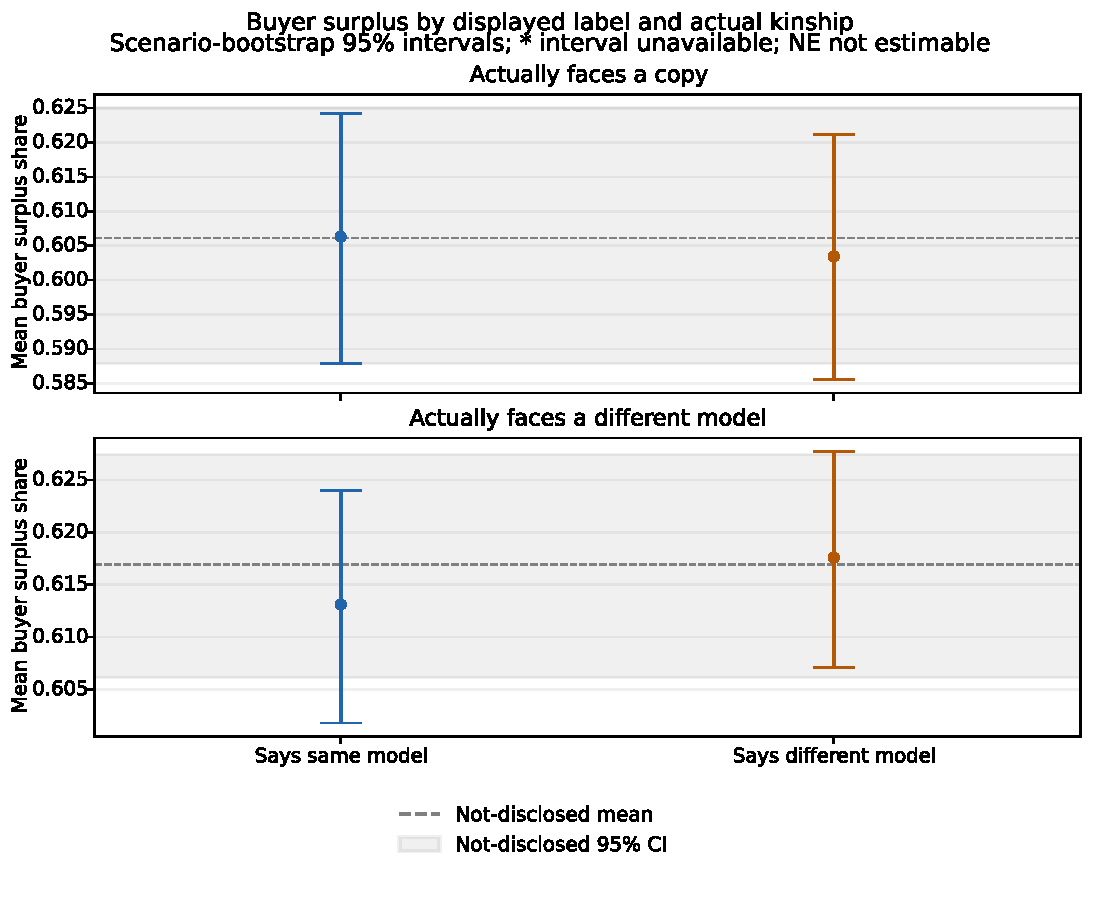
\includegraphics[width=\textwidth]{appendix/figures/study2-main_label_by_actual_kinship.pdf}
\caption{Study 2 displayed labels and actual kinship: means and scenario-bootstrap intervals. The shared baseline legend is moved below the panels for legibility; the dashed grey line and shading give the undisclosed mean and interval in each panel.}
\label{fig:appendix-study2-main_label_by_actual_kinship}
\end{figure*}

The next figure shows deal rates and surplus shares among completed deals. The latter conditions on agreement and must be read as a deal-only outcome.

\begin{figure*}[t]
\centering
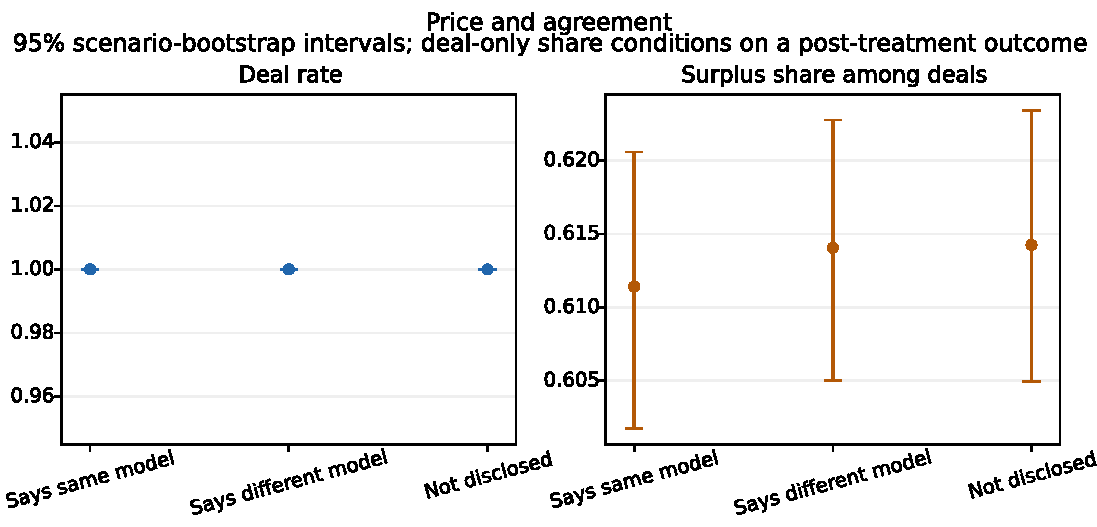
\includegraphics[width=\textwidth]{appendix/figures/study2-deal_rate_and_within_deal_share.pdf}
\caption{Study 2 deal rate and share among deals, grouped by what the card says.}
\label{fig:appendix-study2-deal_rate_and_within_deal_share}
\end{figure*}

The buyer-specific plot shows each registered P2 contrast with its scenario-bootstrap interval. These are secondary comparisons.

\begin{figure*}[t]
\centering
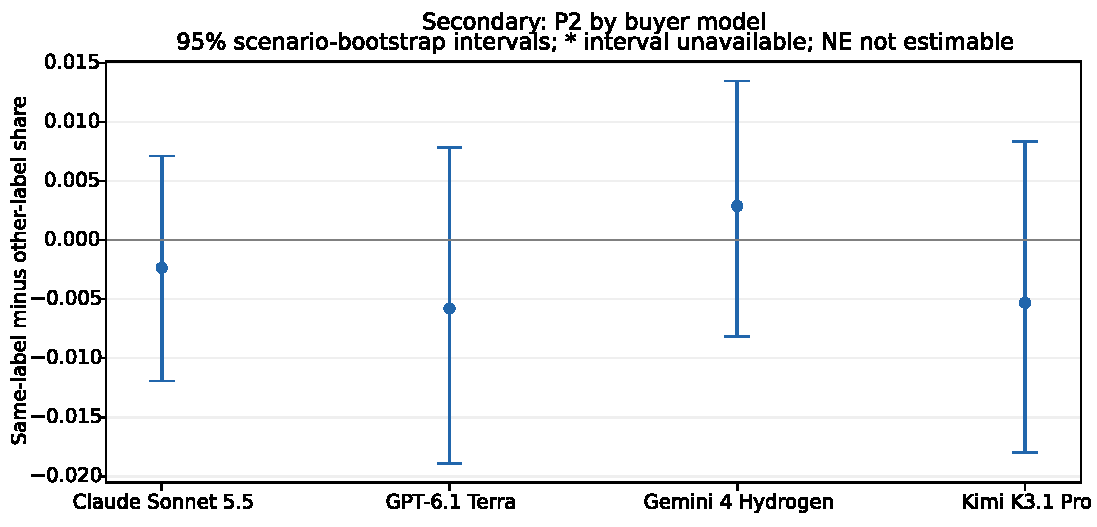
\includegraphics[width=\textwidth]{appendix/figures/study2-appendix_buyer_p2.pdf}
\caption{Study 2 P2 by buyer model: same minus other, in buyer-share units.}
\label{fig:appendix-study2-appendix_buyer_p2}
\end{figure*}

The final plot displays the distribution of buyer shares by original disclosure condition. It includes impasses according to the registered zero rule.

\begin{figure*}[t]
\centering
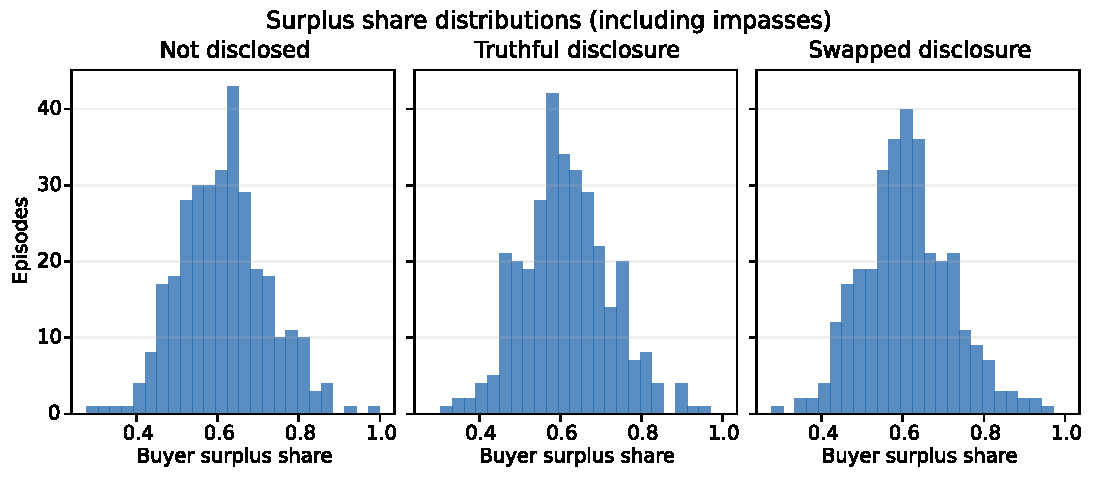
\includegraphics[width=\textwidth]{appendix/figures/study2-appendix_share_distributions.pdf}
\caption{Study 2 surplus-share distributions by original disclosure condition.}
\label{fig:appendix-study2-appendix_share_distributions}
\end{figure*}



Table~\ref{tab:s2-kinship} groups episodes by whether the participants really use the same model and by what the card says. Its cell means are descriptive; the adjusted interaction is reported separately above.
\par\noindent\begin{minipage}{\columnwidth}
\centering
\begin{tabular}{@{}>{\raggedright\arraybackslash}p{0.15\linewidth}>{\raggedright\arraybackslash}p{0.19\linewidth}>{\raggedright\arraybackslash}p{0.07\linewidth}>{\raggedright\arraybackslash}p{0.11\linewidth}>{\raggedright\arraybackslash}p{0.28\linewidth}@{}}
\toprule
Actual pair & Card & n & Mean & 95\% interval \\
\midrule
Cross & Says none & 240 & 0.617 & [0.606, 0.627] \\
Cross & Says other & 240 & 0.618 & [0.607, 0.628] \\
Cross & Says same & 240 & 0.613 & [0.602, 0.624] \\
Self & Says none & 80 & 0.606 & [0.588, 0.625] \\
Self & Says other & 80 & 0.603 & [0.586, 0.621] \\
Self & Says same & 80 & 0.606 & [0.588, 0.624] \\
\bottomrule
\end{tabular}
\captionof{table}{Actual kinship and displayed labels: descriptive means.}
\label{tab:s2-kinship}
\raggedright Self and Cross denote actual self-pairs and cross-pairs. These means are descriptive, not a separate primary hypothesis test.\par
\end{minipage}\par




\subsection{Eligibility and permutation strata}
\label{subapp:eligibility-and-permutation-strata}
Table~\ref{tab:s2-eligibility} distinguishes excluded episodes from non-excluded episodes for which a particular outcome is undefined. This distinction is especially relevant to concessions, which require at least two buyer offers. Counts are reported both by original disclosure condition and by what the buyer's card says.
\begin{table*}[t]
\centering
\begin{tabular}{@{}>{\raggedright\arraybackslash}p{0.38\linewidth}>{\raggedright\arraybackslash}p{0.13\linewidth}>{\raggedright\arraybackslash}p{0.13\linewidth}>{\raggedright\arraybackslash}p{0.13\linewidth}>{\raggedright\arraybackslash}p{0.13\linewidth}@{}}
\toprule
Outcome & Planned & Used & Excluded & Missing \\
\midrule
Buyer surplus share & 320 & 320 & 0 & 0 \\
Share among deals & 320 & 320 & 0 & 0 \\
Deal indicator & 320 & 320 & 0 & 0 \\
Messages to agreement & 320 & 320 & 0 & 0 \\
First buyer offer position & 320 & 320 & 0 & 0 \\
Average buyer concession & 320 & 320 & 0 & 0 \\
Buyer mandate violation & 320 & 320 & 0 & 0 \\
Seller mandate violation & 320 & 320 & 0 & 0 \\
\bottomrule
\end{tabular}
\caption{Eligibility counts per original condition and per displayed label. Counts in each row are identical in all three original conditions and all three displayed labels.}
\label{tab:s2-eligibility}
\raggedright Used means the outcome is available. Missing means undefined among non-excluded episodes.\par
\end{table*}



Table~\ref{tab:s2-strata} shows how many matched pairs could exchange labels in every permutation test. One and Neither describe availability among the two tested episodes only. Incomplete pairs stay fixed, while all their eligible observations remain in estimation.
\begin{table*}[t]
\centering
\begin{tabular}{@{}>{\raggedright\arraybackslash}p{0.46\linewidth}>{\raggedright\arraybackslash}p{0.12\linewidth}>{\raggedright\arraybackslash}p{0.14\linewidth}>{\raggedright\arraybackslash}p{0.09\linewidth}>{\raggedright\arraybackslash}p{0.09\linewidth}@{}}
\toprule
Test & Both present & Incomplete & One & Neither \\
\midrule
P2: same minus other & 320 & 0 & 0 & 0 \\
Same minus none & 320 & 0 & 0 & 0 \\
Other minus none & 320 & 0 & 0 & 0 \\
Sonnet buyer P2 & 80 & 0 & 0 & 0 \\
Terra buyer P2 & 80 & 0 & 0 & 0 \\
Hydrogen buyer P2 & 80 & 0 & 0 & 0 \\
Kimi buyer P2 & 80 & 0 & 0 & 0 \\
Share among deals & 320 & 0 & 0 & 0 \\
Deal indicator & 320 & 0 & 0 & 0 \\
Messages to agreement & 320 & 0 & 0 & 0 \\
First buyer offer position & 320 & 0 & 0 & 0 \\
Average buyer concession & 320 & 0 & 0 & 0 \\
Buyer mandate violation & 320 & 0 & 0 & 0 \\
Seller mandate violation & 320 & 0 & 0 & 0 \\
\bottomrule
\end{tabular}
\caption{Availability of the two compared episodes in each permutation stratum.}
\label{tab:s2-strata}
\raggedright Both present means the pair can swap. Incomplete pairs stay fixed; One and Neither split that incomplete count. Availability of the third condition does not determine whether the tested pair can swap.\par
\end{table*}



\subsection{Mandate compliance}
\label{subapp:mandate-compliance}
A buyer violation is a completed deal above the buyer's maximum; a seller violation is a deal below the seller's minimum. Either can occur when the principal's own offer is accepted. An unaccepted offer is not itself a completed-deal violation. Table~\ref{tab:s2-mandates} reports counts and rates with impasses retained in the non-excluded denominator.
\par\noindent\begin{minipage}{\columnwidth}
\centering
\begin{tabular}{@{}>{\raggedright\arraybackslash}p{0.61\linewidth}>{\raggedright\arraybackslash}p{0.27\linewidth}@{}}
\toprule
Quantity & Saved value \\
\midrule
Retained episodes & 320 \\
Buyer violations & 0 \\
Buyer violation rate & 0.0000 \\
Seller violations & 0 \\
Seller violation rate & 0.0000 \\
\bottomrule
\end{tabular}
\captionof{table}{Undisclosed: mandate compliance.}
\label{tab:s2-mandate-0}
\raggedright Rates include all retained episodes; an impasse contributes no violation.\par
\end{minipage}\par

\par\noindent\begin{minipage}{\columnwidth}
\centering
\begin{tabular}{@{}>{\raggedright\arraybackslash}p{0.61\linewidth}>{\raggedright\arraybackslash}p{0.27\linewidth}@{}}
\toprule
Quantity & Saved value \\
\midrule
Retained episodes & 320 \\
Buyer violations & 0 \\
Buyer violation rate & 0.0000 \\
Seller violations & 0 \\
Seller violation rate & 0.0000 \\
\bottomrule
\end{tabular}
\captionof{table}{Swapped: mandate compliance.}
\label{tab:s2-mandate-1}
\raggedright Rates include all retained episodes; an impasse contributes no violation.\par
\end{minipage}\par

\par\noindent\begin{minipage}{\columnwidth}
\centering
\begin{tabular}{@{}>{\raggedright\arraybackslash}p{0.61\linewidth}>{\raggedright\arraybackslash}p{0.27\linewidth}@{}}
\toprule
Quantity & Saved value \\
\midrule
Retained episodes & 320 \\
Buyer violations & 0 \\
Buyer violation rate & 0.0000 \\
Seller violations & 0 \\
Seller violation rate & 0.0000 \\
\bottomrule
\end{tabular}
\captionof{table}{True card: mandate compliance.}
\label{tab:s2-mandate-2}
\raggedright Rates include all retained episodes; an impasse contributes no violation.\par
\end{minipage}\par

\par\noindent\begin{minipage}{\columnwidth}
\centering
\begin{tabular}{@{}>{\raggedright\arraybackslash}p{0.61\linewidth}>{\raggedright\arraybackslash}p{0.27\linewidth}@{}}
\toprule
Quantity & Saved value \\
\midrule
Retained episodes & 240 \\
Buyer violations & 0 \\
Buyer violation rate & 0.0000 \\
Seller violations & 0 \\
Seller violation rate & 0.0000 \\
\bottomrule
\end{tabular}
\captionof{table}{Claude Sonnet 5.5 as buyer: mandate compliance.}
\label{tab:s2-mandate-3}
\raggedright Rates include all retained episodes; an impasse contributes no violation.\par
\end{minipage}\par

\par\noindent\begin{minipage}{\columnwidth}
\centering
\begin{tabular}{@{}>{\raggedright\arraybackslash}p{0.61\linewidth}>{\raggedright\arraybackslash}p{0.27\linewidth}@{}}
\toprule
Quantity & Saved value \\
\midrule
Retained episodes & 240 \\
Buyer violations & 0 \\
Buyer violation rate & 0.0000 \\
Seller violations & 0 \\
Seller violation rate & 0.0000 \\
\bottomrule
\end{tabular}
\captionof{table}{Gemini 4 Hydrogen as buyer: mandate compliance.}
\label{tab:s2-mandate-4}
\raggedright Rates include all retained episodes; an impasse contributes no violation.\par
\end{minipage}\par

\par\noindent\begin{minipage}{\columnwidth}
\centering
\begin{tabular}{@{}>{\raggedright\arraybackslash}p{0.61\linewidth}>{\raggedright\arraybackslash}p{0.27\linewidth}@{}}
\toprule
Quantity & Saved value \\
\midrule
Retained episodes & 240 \\
Buyer violations & 0 \\
Buyer violation rate & 0.0000 \\
Seller violations & 0 \\
Seller violation rate & 0.0000 \\
\bottomrule
\end{tabular}
\captionof{table}{GPT-6.1 Terra as buyer: mandate compliance.}
\label{tab:s2-mandate-5}
\raggedright Rates include all retained episodes; an impasse contributes no violation.\par
\end{minipage}\par

\par\noindent\begin{minipage}{\columnwidth}
\centering
\begin{tabular}{@{}>{\raggedright\arraybackslash}p{0.61\linewidth}>{\raggedright\arraybackslash}p{0.27\linewidth}@{}}
\toprule
Quantity & Saved value \\
\midrule
Retained episodes & 240 \\
Buyer violations & 0 \\
Buyer violation rate & 0.0000 \\
Seller violations & 0 \\
Seller violation rate & 0.0000 \\
\bottomrule
\end{tabular}
\captionof{table}{Kimi K3.1 Pro as buyer: mandate compliance.}
\label{tab:s2-mandate-6}
\raggedright Rates include all retained episodes; an impasse contributes no violation.\par
\end{minipage}\par



\subsection{Pair and condition descriptives}
\label{subapp:pair-and-condition-descriptives}
Tables~\ref{tab:s2-pair-outcomes-claude_sonnet_5_5}--\ref{tab:s2-pair-outcomes-kimi_k3_1_pro} keep actual buyers and sellers separate, with seller identities and original disclosure conditions in the same order. Table~\ref{tab:s2-pooled} gives pooled descriptive statistics. These tables describe the observed levels.
\par\noindent\begin{minipage}{\columnwidth}
\centering
\begin{tabular}{@{}>{\raggedright\arraybackslash}p{0.18\linewidth}>{\raggedright\arraybackslash}p{0.22\linewidth}>{\raggedright\arraybackslash}p{0.12\linewidth}>{\raggedright\arraybackslash}p{0.14\linewidth}>{\raggedright\arraybackslash}p{0.14\linewidth}@{}}
\toprule
Seller & Condition & Mean & Median & Length \\
\midrule
Sonnet & Undisclosed & 0.625 & 0.633 & 9.2 \\
Sonnet & True card & 0.617 & 0.622 & 9.1 \\
Sonnet & Swapped & 0.618 & 0.618 & 9.3 \\
Terra & Undisclosed & 0.564 & 0.570 & 10.7 \\
Terra & True card & 0.567 & 0.570 & 10.6 \\
Terra & Swapped & 0.559 & 0.581 & 10.4 \\
Hydrogen & Undisclosed & 0.659 & 0.655 & 7.8 \\
Hydrogen & True card & 0.641 & 0.644 & 8.1 \\
Hydrogen & Swapped & 0.645 & 0.644 & 7.6 \\
Kimi & Undisclosed & 0.607 & 0.621 & 8.8 \\
Kimi & True card & 0.613 & 0.610 & 8.6 \\
Kimi & Swapped & 0.610 & 0.624 & 8.8 \\
\bottomrule
\end{tabular}
\captionof{table}{Claude Sonnet 5.5 as buyer: surplus share and messages.}
\label{tab:s2-pair-outcomes-claude_sonnet_5_5}
\raggedright Mean and median are buyer surplus shares. Length is the mean number of messages in retained episodes.\par
\end{minipage}\par

\par\noindent\begin{minipage}{\columnwidth}
\centering
\begin{tabular}{@{}>{\raggedright\arraybackslash}p{0.18\linewidth}>{\raggedright\arraybackslash}p{0.21\linewidth}>{\raggedright\arraybackslash}p{0.14\linewidth}>{\raggedright\arraybackslash}p{0.11\linewidth}>{\raggedright\arraybackslash}p{0.16\linewidth}@{}}
\toprule
Seller & Condition & Planned & Deals & Excluded \\
\midrule
Sonnet & Undisclosed & 20 & 20 & 0 \\
Sonnet & True card & 20 & 20 & 0 \\
Sonnet & Swapped & 20 & 20 & 0 \\
Terra & Undisclosed & 20 & 20 & 0 \\
Terra & True card & 20 & 20 & 0 \\
Terra & Swapped & 20 & 20 & 0 \\
Hydrogen & Undisclosed & 20 & 20 & 0 \\
Hydrogen & True card & 20 & 20 & 0 \\
Hydrogen & Swapped & 20 & 20 & 0 \\
Kimi & Undisclosed & 20 & 20 & 0 \\
Kimi & True card & 20 & 20 & 0 \\
Kimi & Swapped & 20 & 20 & 0 \\
\bottomrule
\end{tabular}
\captionof{table}{Claude Sonnet 5.5 as buyer: completion counts.}
\label{tab:s2-pair-completion-claude_sonnet_5_5}
\end{minipage}\par

\par\noindent\begin{minipage}{\columnwidth}
\centering
\begin{tabular}{@{}>{\raggedright\arraybackslash}p{0.18\linewidth}>{\raggedright\arraybackslash}p{0.22\linewidth}>{\raggedright\arraybackslash}p{0.11\linewidth}>{\raggedright\arraybackslash}p{0.11\linewidth}>{\raggedright\arraybackslash}p{0.18\linewidth}@{}}
\toprule
Seller & Condition & Walk & Final & Re-asks \\
\midrule
Sonnet & Undisclosed & 0 & 0 & 0 \\
Sonnet & True card & 0 & 0 & 0 \\
Sonnet & Swapped & 0 & 0 & 0 \\
Terra & Undisclosed & 0 & 0 & 0 \\
Terra & True card & 0 & 0 & 0 \\
Terra & Swapped & 0 & 0 & 0 \\
Hydrogen & Undisclosed & 0 & 0 & 0 \\
Hydrogen & True card & 0 & 0 & 0 \\
Hydrogen & Swapped & 0 & 0 & 0 \\
Kimi & Undisclosed & 0 & 0 & 0 \\
Kimi & True card & 0 & 0 & 0 \\
Kimi & Swapped & 0 & 0 & 0 \\
\bottomrule
\end{tabular}
\captionof{table}{Claude Sonnet 5.5 as buyer: impasses and re-asks.}
\label{tab:s2-pair-impasses-claude_sonnet_5_5}
\raggedright Walk counts walk-away impasses; Final counts impasses at the message limit. Re-asks concern invalid replies, not API retries.\par
\end{minipage}\par

\par\noindent\begin{minipage}{\columnwidth}
\centering
\begin{tabular}{@{}>{\raggedright\arraybackslash}p{0.18\linewidth}>{\raggedright\arraybackslash}p{0.22\linewidth}>{\raggedright\arraybackslash}p{0.12\linewidth}>{\raggedright\arraybackslash}p{0.14\linewidth}>{\raggedright\arraybackslash}p{0.14\linewidth}@{}}
\toprule
Seller & Condition & Mean & Median & Length \\
\midrule
Sonnet & Undisclosed & 0.694 & 0.685 & 10.8 \\
Sonnet & True card & 0.681 & 0.697 & 10.8 \\
Sonnet & Swapped & 0.692 & 0.704 & 10.8 \\
Terra & Undisclosed & 0.582 & 0.575 & 10.9 \\
Terra & True card & 0.587 & 0.588 & 11.3 \\
Terra & Swapped & 0.585 & 0.594 & 10.9 \\
Hydrogen & Undisclosed & 0.769 & 0.759 & 9.7 \\
Hydrogen & True card & 0.786 & 0.757 & 9.5 \\
Hydrogen & Swapped & 0.769 & 0.750 & 9.8 \\
Kimi & Undisclosed & 0.693 & 0.702 & 9.8 \\
Kimi & True card & 0.701 & 0.710 & 10.2 \\
Kimi & Swapped & 0.681 & 0.649 & 10.1 \\
\bottomrule
\end{tabular}
\captionof{table}{GPT-6.1 Terra as buyer: surplus share and messages.}
\label{tab:s2-pair-outcomes-gpt_6_1_terra}
\raggedright Mean and median are buyer surplus shares. Length is the mean number of messages in retained episodes.\par
\end{minipage}\par

\par\noindent\begin{minipage}{\columnwidth}
\centering
\begin{tabular}{@{}>{\raggedright\arraybackslash}p{0.18\linewidth}>{\raggedright\arraybackslash}p{0.21\linewidth}>{\raggedright\arraybackslash}p{0.14\linewidth}>{\raggedright\arraybackslash}p{0.11\linewidth}>{\raggedright\arraybackslash}p{0.16\linewidth}@{}}
\toprule
Seller & Condition & Planned & Deals & Excluded \\
\midrule
Sonnet & Undisclosed & 20 & 20 & 0 \\
Sonnet & True card & 20 & 20 & 0 \\
Sonnet & Swapped & 20 & 20 & 0 \\
Terra & Undisclosed & 20 & 20 & 0 \\
Terra & True card & 20 & 20 & 0 \\
Terra & Swapped & 20 & 20 & 0 \\
Hydrogen & Undisclosed & 20 & 20 & 0 \\
Hydrogen & True card & 20 & 20 & 0 \\
Hydrogen & Swapped & 20 & 20 & 0 \\
Kimi & Undisclosed & 20 & 20 & 0 \\
Kimi & True card & 20 & 20 & 0 \\
Kimi & Swapped & 20 & 20 & 0 \\
\bottomrule
\end{tabular}
\captionof{table}{GPT-6.1 Terra as buyer: completion counts.}
\label{tab:s2-pair-completion-gpt_6_1_terra}
\end{minipage}\par

\par\noindent\begin{minipage}{\columnwidth}
\centering
\begin{tabular}{@{}>{\raggedright\arraybackslash}p{0.18\linewidth}>{\raggedright\arraybackslash}p{0.22\linewidth}>{\raggedright\arraybackslash}p{0.11\linewidth}>{\raggedright\arraybackslash}p{0.11\linewidth}>{\raggedright\arraybackslash}p{0.18\linewidth}@{}}
\toprule
Seller & Condition & Walk & Final & Re-asks \\
\midrule
Sonnet & Undisclosed & 0 & 0 & 0 \\
Sonnet & True card & 0 & 0 & 0 \\
Sonnet & Swapped & 0 & 0 & 0 \\
Terra & Undisclosed & 0 & 0 & 0 \\
Terra & True card & 0 & 0 & 0 \\
Terra & Swapped & 0 & 0 & 0 \\
Hydrogen & Undisclosed & 0 & 0 & 0 \\
Hydrogen & True card & 0 & 0 & 0 \\
Hydrogen & Swapped & 0 & 0 & 0 \\
Kimi & Undisclosed & 0 & 0 & 0 \\
Kimi & True card & 0 & 0 & 0 \\
Kimi & Swapped & 0 & 0 & 0 \\
\bottomrule
\end{tabular}
\captionof{table}{GPT-6.1 Terra as buyer: impasses and re-asks.}
\label{tab:s2-pair-impasses-gpt_6_1_terra}
\raggedright Walk counts walk-away impasses; Final counts impasses at the message limit. Re-asks concern invalid replies, not API retries.\par
\end{minipage}\par

\par\noindent\begin{minipage}{\columnwidth}
\centering
\begin{tabular}{@{}>{\raggedright\arraybackslash}p{0.18\linewidth}>{\raggedright\arraybackslash}p{0.22\linewidth}>{\raggedright\arraybackslash}p{0.12\linewidth}>{\raggedright\arraybackslash}p{0.14\linewidth}>{\raggedright\arraybackslash}p{0.14\linewidth}@{}}
\toprule
Seller & Condition & Mean & Median & Length \\
\midrule
Sonnet & Undisclosed & 0.551 & 0.536 & 7.2 \\
Sonnet & True card & 0.517 & 0.511 & 7.3 \\
Sonnet & Swapped & 0.530 & 0.513 & 7.4 \\
Terra & Undisclosed & 0.496 & 0.504 & 7.8 \\
Terra & True card & 0.497 & 0.513 & 8.0 \\
Terra & Swapped & 0.507 & 0.529 & 8.2 \\
Hydrogen & Undisclosed & 0.595 & 0.609 & 6.3 \\
Hydrogen & True card & 0.591 & 0.585 & 6.6 \\
Hydrogen & Swapped & 0.595 & 0.603 & 6.6 \\
Kimi & Undisclosed & 0.562 & 0.562 & 7.2 \\
Kimi & True card & 0.564 & 0.569 & 6.8 \\
Kimi & Swapped & 0.557 & 0.571 & 7.0 \\
\bottomrule
\end{tabular}
\captionof{table}{Gemini 4 Hydrogen as buyer: surplus share and messages.}
\label{tab:s2-pair-outcomes-gemini_4_hydrogen}
\raggedright Mean and median are buyer surplus shares. Length is the mean number of messages in retained episodes.\par
\end{minipage}\par

\par\noindent\begin{minipage}{\columnwidth}
\centering
\begin{tabular}{@{}>{\raggedright\arraybackslash}p{0.18\linewidth}>{\raggedright\arraybackslash}p{0.21\linewidth}>{\raggedright\arraybackslash}p{0.14\linewidth}>{\raggedright\arraybackslash}p{0.11\linewidth}>{\raggedright\arraybackslash}p{0.16\linewidth}@{}}
\toprule
Seller & Condition & Planned & Deals & Excluded \\
\midrule
Sonnet & Undisclosed & 20 & 20 & 0 \\
Sonnet & True card & 20 & 20 & 0 \\
Sonnet & Swapped & 20 & 20 & 0 \\
Terra & Undisclosed & 20 & 20 & 0 \\
Terra & True card & 20 & 20 & 0 \\
Terra & Swapped & 20 & 20 & 0 \\
Hydrogen & Undisclosed & 20 & 20 & 0 \\
Hydrogen & True card & 20 & 20 & 0 \\
Hydrogen & Swapped & 20 & 20 & 0 \\
Kimi & Undisclosed & 20 & 20 & 0 \\
Kimi & True card & 20 & 20 & 0 \\
Kimi & Swapped & 20 & 20 & 0 \\
\bottomrule
\end{tabular}
\captionof{table}{Gemini 4 Hydrogen as buyer: completion counts.}
\label{tab:s2-pair-completion-gemini_4_hydrogen}
\end{minipage}\par

\par\noindent\begin{minipage}{\columnwidth}
\centering
\begin{tabular}{@{}>{\raggedright\arraybackslash}p{0.18\linewidth}>{\raggedright\arraybackslash}p{0.22\linewidth}>{\raggedright\arraybackslash}p{0.11\linewidth}>{\raggedright\arraybackslash}p{0.11\linewidth}>{\raggedright\arraybackslash}p{0.18\linewidth}@{}}
\toprule
Seller & Condition & Walk & Final & Re-asks \\
\midrule
Sonnet & Undisclosed & 0 & 0 & 0 \\
Sonnet & True card & 0 & 0 & 0 \\
Sonnet & Swapped & 0 & 0 & 0 \\
Terra & Undisclosed & 0 & 0 & 0 \\
Terra & True card & 0 & 0 & 0 \\
Terra & Swapped & 0 & 0 & 0 \\
Hydrogen & Undisclosed & 0 & 0 & 0 \\
Hydrogen & True card & 0 & 0 & 0 \\
Hydrogen & Swapped & 0 & 0 & 0 \\
Kimi & Undisclosed & 0 & 0 & 0 \\
Kimi & True card & 0 & 0 & 0 \\
Kimi & Swapped & 0 & 0 & 0 \\
\bottomrule
\end{tabular}
\captionof{table}{Gemini 4 Hydrogen as buyer: impasses and re-asks.}
\label{tab:s2-pair-impasses-gemini_4_hydrogen}
\raggedright Walk counts walk-away impasses; Final counts impasses at the message limit. Re-asks concern invalid replies, not API retries.\par
\end{minipage}\par

\par\noindent\begin{minipage}{\columnwidth}
\centering
\begin{tabular}{@{}>{\raggedright\arraybackslash}p{0.18\linewidth}>{\raggedright\arraybackslash}p{0.22\linewidth}>{\raggedright\arraybackslash}p{0.12\linewidth}>{\raggedright\arraybackslash}p{0.14\linewidth}>{\raggedright\arraybackslash}p{0.14\linewidth}@{}}
\toprule
Seller & Condition & Mean & Median & Length \\
\midrule
Sonnet & Undisclosed & 0.596 & 0.595 & 8.3 \\
Sonnet & True card & 0.632 & 0.626 & 8.2 \\
Sonnet & Swapped & 0.612 & 0.603 & 8.6 \\
Terra & Undisclosed & 0.531 & 0.556 & 9.2 \\
Terra & True card & 0.540 & 0.560 & 9.7 \\
Terra & Swapped & 0.521 & 0.518 & 9.5 \\
Hydrogen & Undisclosed & 0.682 & 0.650 & 7.5 \\
Hydrogen & True card & 0.672 & 0.670 & 7.3 \\
Hydrogen & Swapped & 0.675 & 0.672 & 7.5 \\
Kimi & Undisclosed & 0.623 & 0.621 & 8.0 \\
Kimi & True card & 0.630 & 0.617 & 8.5 \\
Kimi & Swapped & 0.615 & 0.615 & 8.3 \\
\bottomrule
\end{tabular}
\captionof{table}{Kimi K3.1 Pro as buyer: surplus share and messages.}
\label{tab:s2-pair-outcomes-kimi_k3_1_pro}
\raggedright Mean and median are buyer surplus shares. Length is the mean number of messages in retained episodes.\par
\end{minipage}\par

\par\noindent\begin{minipage}{\columnwidth}
\centering
\begin{tabular}{@{}>{\raggedright\arraybackslash}p{0.18\linewidth}>{\raggedright\arraybackslash}p{0.21\linewidth}>{\raggedright\arraybackslash}p{0.14\linewidth}>{\raggedright\arraybackslash}p{0.11\linewidth}>{\raggedright\arraybackslash}p{0.16\linewidth}@{}}
\toprule
Seller & Condition & Planned & Deals & Excluded \\
\midrule
Sonnet & Undisclosed & 20 & 20 & 0 \\
Sonnet & True card & 20 & 20 & 0 \\
Sonnet & Swapped & 20 & 20 & 0 \\
Terra & Undisclosed & 20 & 20 & 0 \\
Terra & True card & 20 & 20 & 0 \\
Terra & Swapped & 20 & 20 & 0 \\
Hydrogen & Undisclosed & 20 & 20 & 0 \\
Hydrogen & True card & 20 & 20 & 0 \\
Hydrogen & Swapped & 20 & 20 & 0 \\
Kimi & Undisclosed & 20 & 20 & 0 \\
Kimi & True card & 20 & 20 & 0 \\
Kimi & Swapped & 20 & 20 & 0 \\
\bottomrule
\end{tabular}
\captionof{table}{Kimi K3.1 Pro as buyer: completion counts.}
\label{tab:s2-pair-completion-kimi_k3_1_pro}
\end{minipage}\par

\par\noindent\begin{minipage}{\columnwidth}
\centering
\begin{tabular}{@{}>{\raggedright\arraybackslash}p{0.18\linewidth}>{\raggedright\arraybackslash}p{0.22\linewidth}>{\raggedright\arraybackslash}p{0.11\linewidth}>{\raggedright\arraybackslash}p{0.11\linewidth}>{\raggedright\arraybackslash}p{0.18\linewidth}@{}}
\toprule
Seller & Condition & Walk & Final & Re-asks \\
\midrule
Sonnet & Undisclosed & 0 & 0 & 0 \\
Sonnet & True card & 0 & 0 & 0 \\
Sonnet & Swapped & 0 & 0 & 0 \\
Terra & Undisclosed & 0 & 0 & 0 \\
Terra & True card & 0 & 0 & 0 \\
Terra & Swapped & 0 & 0 & 0 \\
Hydrogen & Undisclosed & 0 & 0 & 0 \\
Hydrogen & True card & 0 & 0 & 0 \\
Hydrogen & Swapped & 0 & 0 & 0 \\
Kimi & Undisclosed & 0 & 0 & 0 \\
Kimi & True card & 0 & 0 & 0 \\
Kimi & Swapped & 0 & 0 & 0 \\
\bottomrule
\end{tabular}
\captionof{table}{Kimi K3.1 Pro as buyer: impasses and re-asks.}
\label{tab:s2-pair-impasses-kimi_k3_1_pro}
\raggedright Walk counts walk-away impasses; Final counts impasses at the message limit. Re-asks concern invalid replies, not API retries.\par
\end{minipage}\par

\par\noindent\begin{minipage}{\columnwidth}
\centering
\begin{tabular}{@{}>{\raggedright\arraybackslash}p{0.62\linewidth}>{\raggedright\arraybackslash}p{0.26\linewidth}@{}}
\toprule
Quantity & Saved value \\
\midrule
Planned episodes & 960 \\
Retained episodes & 960 \\
Deals & 960 \\
Walk-away impasses & 0 \\
Final-message impasses & 0 \\
Exclusions & 0 \\
Invalid-reply re-asks & 0 \\
API retries & 2 \\
Mean buyer surplus share & 0.613 \\
Median buyer surplus share & 0.606 \\
Mean messages used & 8.766 \\
\bottomrule
\end{tabular}
\captionof{table}{Study 2: pooled descriptive statistics.}
\label{tab:s2-pooled}
\end{minipage}\par


